Una prueba de conocimiento cero permite probar la verdad de una declaración sin compartir el contenido de la declaración o revelar cómo descubrió la verdad. Para que esto sea posible, los protocolos de conocimiento cero se basan en algoritmos que toman algunos datos como entrada y devuelven ``verdadero'' o ``falso'' como salida.

Se utiliza una serie de algoritmos criptográficos en las aplicaciones del mundo real de los ZKP para permitir la verificación de una declaración computacional. Por ejemplo, utilizando métodos ZKP, un receptor de pago puede verificar que el pagador tiene suficiente saldo en su cuenta bancaria sin obtener ninguna otra información sobre el saldo del pagador.

Un protocolo de conocimiento cero debe satisfacer los siguientes criterios:
\begin{itemize}
    \item Completitud (\emph{Completeness}): Si la entrada es válida, el protocolo de conocimiento cero siempre devuelve ``verdadero". Por lo tanto, si la declaración subyacente es verdadera y el probador y el verificador actúan honestamente, la prueba puede ser aceptada.

    \item Solidez (\emph{Soundness}): Si la entrada no es válida, es teóricamente imposible engañar al protocolo de conocimiento cero para que devuelva ``verdadero". Por lo tanto, un probador mentiroso no puede engañar a un verificador honesto para que crea que una declaración inválida es válida (excepto con un pequeño margen de probabilidad).

    \item Conocimiento cero (\emph{Zero-knowledge}): El verificador no aprende nada sobre una declaración más allá de su validez o falsedad (tiene ``conocimiento cero" de la declaración). Este requisito también evita que el verificador derive la entrada original (el contenido de la declaración) de la prueba.
\end{itemize}

El esquema de un protocolo de conocimiento cero queda resumido en la \autoref{im:zkp}:
\begin{figure}[ht]
    \centering
    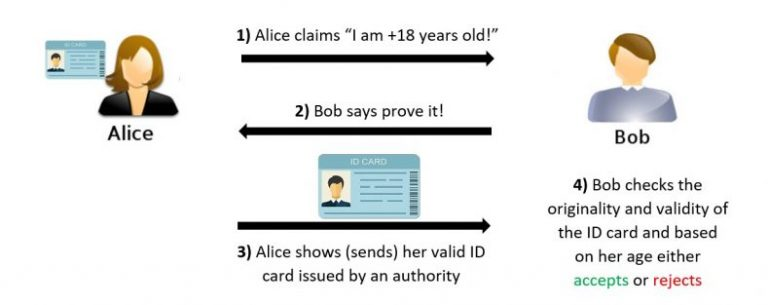
\includegraphics[width=\textwidth]{images/zkp.jpg}
    \caption{Esquema de ZKP \cite{ZKP}}
    \label{im:zkp}
\end{figure}

\section{Clases de protocolos de conocimiento cero} \label{sec:clases}

Lo anterior describe la estructura de una \textbf{prueba interactiva de conocimiento cero}. Los primeros protocolos de conocimiento cero usaban pruebas interactivas, donde verificar la validez de una declaración requería una comunicación de ida y vuelta entre probadores y verificadores.

Esta prueba interactiva tiene una utilidad limitada, ya que requiere que las dos partes estén disponibles e interactúen repetidamente. Incluso si un verificador está convencido de la honestidad de un probador, la prueba no está disponible para una verificación independiente (el cálculo de una nueva prueba requiere un nuevo conjunto de mensajes entre el probador y el verificador).

Para resolver este problema, surgen las \textbf{pruebas de conocimiento cero no interactivas} donde el probador y el verificador tienen una clave compartida. Esto permite que el probador demuestre su conocimiento de cierta información (es decir, testigo) sin proporcionar la información en sí.

A diferencia de las pruebas interactivas, las pruebas no interactivas requieren sólo una ronda de comunicación entre los participantes (proveedor y verificador). El probador pasa la información secreta a un algoritmo especial para calcular una prueba de conocimiento cero. Esta prueba se envía al verificador, quien comprueba que el probador conoce la información secreta utilizando otro algoritmo.

La prueba no interactiva reduce la comunicación entre el probador y el verificador, lo que hace que las pruebas de conocimiento cero sean más eficientes. Además, una vez que se genera una prueba, está disponible para que cualquier otra persona (con acceso al algoritmo de verificación) la verifique.

Las pruebas de conocimiento cero pueden expresarse de la siguiente forma: Dado un elemento $x$ de un lenguaje $\mathcal{L} \in NP$ , una entidad llamada probador es capaz de convencer a un verificador de que $x$ pertenece efectivamente a $\mathcal{L}$, es decir, existe un testigo $w$ para $x$.

Un esquema de prueba de conocimiento cero no interactivo (NIZK) se define mediante los algoritmos de configuración, prueba y verificación de la siguiente manera:
\begin{itemize}
    \item El algoritmo de configuración (\emph{Setup}): Es responsable de la generación de parámetros. Concretamente, tenemos que $params = Setup(\lambda)$, donde la entrada es el parámetro de seguridad $\lambda$ y la salida son los parámetros del sistema de algoritmos ZKP.

    \item La sintaxis de prueba (\emph{Prove}): Viene dada por $\operatorname{proof} = \operatorname{Prove}(x, w)$. El algoritmo recibe como entrada una instancia $x$ de algún lenguaje NP $\mathcal{L}$, y el testigo w, y genera la prueba de conocimiento cero.

    \item El algoritmo de verificación (\emph{Verify}): Recibe la prueba $\operatorname{proof}$ como entrada $y$ genera un bit b, que es igual a 1 si el verificador acepta la prueba, o 0 si la rechaza.
\end{itemize}

Con estos términos, los criterios vistos previamente se pueden expresar de la siguiente forma:
\begin{itemize}
    \item Completitud (\emph{Completeness}): Acepta si la entrada es verdadera, es decir, dado un testigo $w$ que satisface la instancia $x$, tenemos que
    $$\operatorname{Verify}(\operatorname{Prove}(x, w)) = 1$$

    \item Solidez (\emph{Soundness}): Si la entrada no es válida, rechaza excepto con un pequeño margen de error; es decir, si el testigo $w$ no satisface $x$, entonces la probabilidad
    $$P[\operatorname{Verify}(\operatorname{Prove}(x, w)) = 1]$$
    es suficientemente baja.

    \item Conocimiento cero (\emph{Zero-knowledge}): El verificador no aprende nada sobre una declaración más allá de su validez o falsedad. Para ello, dada la interacción entre el probador y el verificador, llamamos a esta interacción una vista, y para capturar la propiedad de conocimiento cero, usamos un simulador de tiempo polinomial, que tiene acceso a la misma entrada proporcionada al verificador (incluida su aleatoriedad), pero no acceso a la entrada del probador, para generar una vista simulada. Decimos que el esquema ZKP tiene conocimiento cero perfecto si la vista simulada, bajo el supuesto de que $x \in \mathcal{L}$, tiene la misma distribución que la vista original. Decimos que el esquema ZKP tiene conocimiento estadístico cero si esas distribuciones son estadísticamente cercanas. Decimos que el esquema ZKP tiene conocimiento computacional cero si no hay un distintivo de tiempo polinomial para esas distribuciones. Intuitivamente, la existencia de un simulador de este tipo significa que cualquier cosa que el verificador pueda calcular a partir de la interacción con el probador, ya era posible calcularla antes de tal interacción, por lo que el verificador no aprendió nada de ella. Además, decimos que es una prueba de conocimiento si podemos encontrar un extractor, que tiene acceso de caja negra rebobinable al probador, que puede calcular el testigo $w$ con una probabilidad no despreciable.
\end{itemize}

\section{Algoritmos basados en ZKP}

ZK-SNARK es un acrónimo de \textit{Zero-Knowledge Succinct Non-Interactive Argument of Knowledge}. El protocolo ZK-SNARK tiene las siguientes cualidades:
\begin{itemize}
    \item Conocimiento cero (\emph{Zero-knowledge}): Un verificador puede validar la integridad de una declaración sin saber nada más sobre la declaración. El único conocimiento que tiene el verificador de la declaración es si es verdadera o falsa.

     \item Sucinto (\emph{Succinct}): La prueba de conocimiento cero es más pequeña que el testigo y se puede verificar rápidamente.

     \item No interactivo (\emph{Non-interactive}): La prueba es ``no interactiva" porque el probador y el verificador solo interactúan una vez, a diferencia de las pruebas interactivas que requieren múltiples rondas de comunicación.

     \item Argumento (\emph{Argument}): La prueba satisface el requisito de ``solidez", por lo que es extremadamente improbable hacer trampa.

     \item De conocimiento (\emph{Of Knowledge}): La prueba de conocimiento cero no puede construirse sin acceso a la información secreta (testigo). Es difícil, si no imposible, para un probador que no tiene el testigo calcular una prueba válida de conocimiento cero.
\end{itemize}

ZK-STARK es un acrónimo de Zero-Knowledge Scalable Transparent Argument of Knowledge. Los ZK-STARK son similares a los ZK-SNARK. Sin embargo añade las siguientes cualidades:
\begin{itemize}
    \item Escalable (\emph{Scalable}): ZK-STARK es más rápido que ZK-SNARK en la generación y verificación de pruebas cuando el tamaño del testigo es mayor. Con las pruebas STARK, los tiempos de prueba y verificación solo aumentan ligeramente a medida que crece el testigo (los tiempos de prueba y verificación de SNARK aumentan linealmente con el tamaño del testigo).
     
     \item Transparente (\emph{Transparent}): ZK-STARK se basa en la aleatoriedad verificable públicamente para generar parámetros públicos para probar y verificar en lugar de una configuración confiable. Por lo tanto, son más transparentes en comparación con los ZK-SNARK.
\end{itemize}

\begin{figure}[ht]
    \centering
    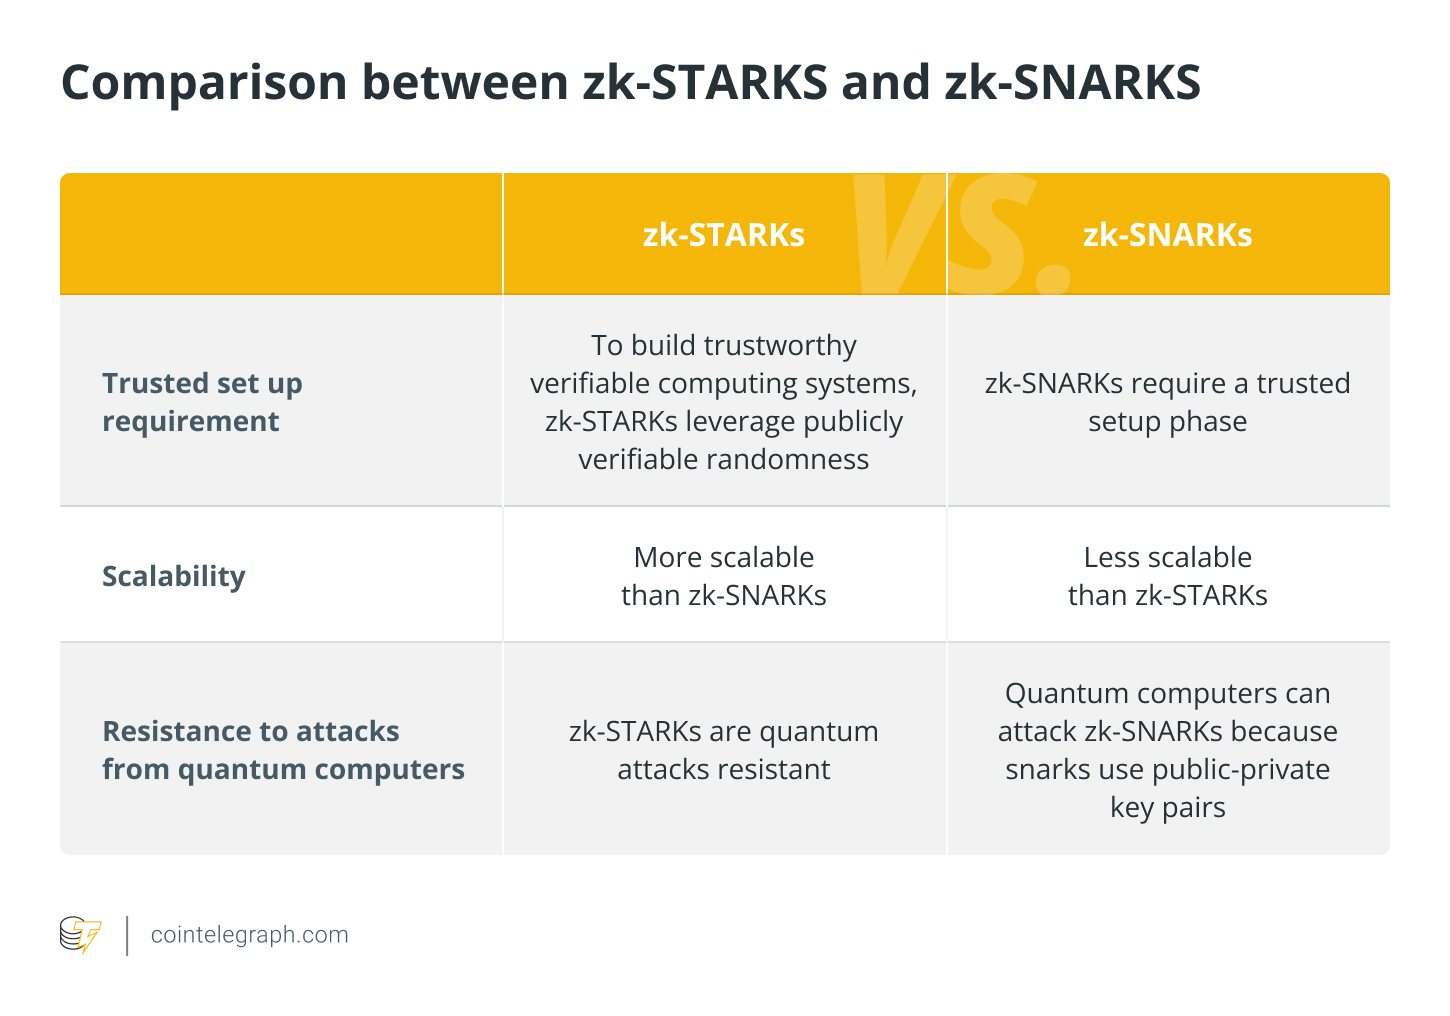
\includegraphics[width=0.7\textwidth]{images/zkstarks vs zksnarks.jpg}
    \caption{ZK-STARK vs ZK-SNARK \cite{zk-STARKs vs zk-SNARKs}}
    \label{im:zkstarks vs zksnarks}
\end{figure}

Los ZK-STARK producen pruebas más grandes que los ZK-SNARK, lo que significa que generalmente tienen gastos generales de verificación más altos. Sin embargo, hay casos (como probar grandes conjuntos de datos) en los que los ZK-STARK pueden ser más rentables que los ZK-SNARK.

Finalmente, como caso particular de los algoritmos de cero conocimiento tenemos las prueba de rango de conocimiento cero (\emph{Zero Knowledge Range Proof}), que permiten probar que un valor entero secreto pertenece a un intervalo. Por ejemplo, si definimos el intervalo como todos los enteros entre 18 y 200, una persona puede usar ZKRP para probar que es mayor de edad.

En este trabajo, nos centraremos en algoritmos de este último tipo, en el que el probador quiere demostrar que conoce un valor secreto que pertenece a un intervalo.

\section{Algoritmos ZKRP}

Este trabajo se va a centrar en el estudio de una prueba de rango de conocimiento cero que será implementada para la herramienta docente. Esta prueba va a ser la Descomposición cuadrada (\emph{Square Decomposition}), elección que se justificará más adelante en la sección \nameref{sec:seleccion}. Debido a esto, aunque se comenten las distintas pruebas que existen, se entrará más en detalle y se añadirán ejemplos numéricos exclusivamente de este algoritmo.

Las ZKRP pueden clasificarse en:
\begin{itemize}
    \item Propuestas de representación entera:
    \begin{itemize}
        \item Descomposición cuadrada (\emph{Square decomposition}): 
        Una de las ideas que se pueden utilizar para obtener pruebas de rango de conocimiento cero es la descomposición del elemento secreto en una suma de cuadrados. Para probar que $x \in [a, b]$ es equivalente a probar que $x - a \geq 0$ y que $b - x \geq 0$.

        Entonces, si podemos probar que $x - a$ y $b - x$ se pueden expresar como cuadrados con una cierta tolerancia $\theta$, estaremos probando que son positivos y, por lo tanto, que el secreto $x$ pertenece al intervalo $[a, b]$.

        El problema de este procedimiento es que es de tiempo $\mathcal{O}(k^{4})$, donde $k$ es el tamaño del elemento secreto, por lo que suele provocar un mal rendimiento con pruebas de tamaño elevado.
        
        \item Basado en firma (\emph{Signature-based}):
        Inicialmente, todos los elementos en el intervalo están firmados, y la prueba de que el probador conoce la firma significa que este número entero pertenece al intervalo esperado, que puede ser cualquier conjunto finito posible.
    \end{itemize}
    \item Propuestas de representación binaria:
    \begin{itemize}
        \item Decomposición multi-base (\emph{Multi-base decomposition}):
        Consiste en descomponer el elemento secreo en la representación binaria, lo que permite probar que pertenece al intervalo usando aritmética booleana. El probador tiene que proveer una prueba \emph{zero knowledge} de que cada bit del elemento secreto es de hecho un bit, y que la representación es válida. En lugar de una descomposición en bits, podemos usar una representación u-aria, obteniendo una mayor eficiencia.
        
        \item Compromisos homomórficos de dos niveles (\emph{Two-tiered homomorphic commitments}):
        Se basa en un argumento para multiplicación en \emph{batches} de elementos de $\mathbb{Z}_{p}$, que puede ser usado para probar que $u_{i}v_{i} = w_{i}$, con $u_{i}, v_{i}, w_{i} \in \mathbb{Z}_{p}$ para $0 < i < N$, siendo $N$ la longitud en bits del secreto. Para construir ZKRP, si los bits del secreto están dados por $w_{i}$, entonces el argumento puede usarse para mostrar que $w_{i}w_{i} = w_{i}$, lo que demuestra al verificador de que, de hecho, $w_{i} \in \{0, 1\}$. Además, mostró cómo probar que $w = \sum_{i=0}^{N} w_{i} 2^{i}$, demostrando así $w \in [0,2^{N})$. El argumento se puede adaptar fácilmente a un intervalo general $[A, B)$. La idea clave de la construcción de Groth es utilizar emparejamientos bilineales para comprometerse con un vector de compromisos de Pedersen. Por ejemplo, dado el emparejamiento $e: \mathbb{G}_{1} \times \mathbb{G}_{2} \to \mathbb{G}_{T}$ y los elementos $v, u_{1}, \dots, u_{N} \in \mathbb{G}{2}$, podemos comprometernos con el vector $[c_{1}, \dots, c_{N}] \in \mathbb{G}_{1}^{n}$ eligiendo un número aleatorio $t \in \mathbb{G}$ y calculando $C = e(t, v) \prod_{i=0}^{N} e(c_{i}, u_{i})$.
        
        \item Bulletproofs: Todos los algoritmos mencionados anteriormente dependen de una configuración confiable, lo que es un problema en el contexto de las criptomonedas, ya que si un adversario puede evitar esta configuración confiable, podría crear dinero de la nada. Recientemente, en 2017, \emph{Stanford Applied Cryptography Group} propuso una nueva idea para construir ZKRP, llamada Bulletproofs. Consiste en utilizar una prueba interna del producto para lograr ZKRP con tamaños de prueba muy pequeños.
        
        En resumen, utilizando este protocolo ZKP, el probador convence a un verificador de que conoce vectores cuyo producto interno es igual a un valor público determinado.
    \end{itemize}
\end{itemize}

A continuación se desarrollan, explicando su funcionamiento, los algoritmos de representación entera (Descomposición Cuadrada y Basados en firmas) y el más relevante de representación binaria, \emph{Bulletproofs}. Como se comentó previamente, este trabajo se centrará en la Descomposición Cuadrada, por lo que será el que se desarrollará en más detalle. Los \emph{Bulletproofs}, al ser el único que se detalla de representación binaria, también estará algo más extendido. Finalmente, los Basados en firmas se comentarán para tener un algoritmo de representación entera con el que poder comparar el funcionamiento, por lo que sólo se hará un breve resumen al respecto.

\subsection{Descomposición cuadrada (\emph{Square decomposition})}

Vamos a estudiar la Descomposición cuadrada en más detalle, desarrollándo en más detalle su funcionamiento. Para ello, añadiremos los distintos algoritmos que utiliza, así como ejemplos numéricos que faciliten su entendimiento. Además, desarrollaremos algunos de los conceptos matemáticos en los que se basa dicho algoritmo.

Sea un entero positivo $x$, y sea $E = g^{x}h^{r} (\operatorname{mod} \text{ n})$, y supongamos que Alice quiere probar a Bob que $x \in [a, b]$.

Inicialmente, Alice escribe el entero positivo $x-a$ como la suma de $x_{1}^{2}$, el cuadrado mayor menor que $x$, y de $\rho$, un número positivo menor que $2\sqrt{x-a}$. Luego, selecciona aleatoriamente $r_{1}, r_{2}$ en $[0, 2^{s}n-1]$ de modo que $r_{1} + r_{2} = r$ y calcula $E_{1} = g^{x_{1}^{2}}h^{r{1}}$ y $E_{2} = g^{\rho}h^{r_{2}}$. Lee demuestra a Bob que $E_{1}$ oculta un cuadrado y que $E_{2}$ oculta un número cuyo valor absoluto es menor que $2^{t+\ell+1}\sqrt{b-a}$ mediante una prueba CFT. Finalmente, aplica el mismo método a $b-x$. Esto conduce a una demostración de que $x \in [a - 2^{t+\ell+1}\sqrt{b-a}, b + 2^{t+\ell+1}\sqrt{b-a}]$. La tasa de expansión de esta prueba es igual a $1 + (2^{t+\ell+1}/\sqrt{b-a})$, que se acerca a $1$ cuando $b-a$ es grande.

Luego, aumentamos artificialmente el tamaño de $x$ estableciendo $x' = 2^{T}x$. Usando el esquema anterior, demostramos que $x' \in [2^{T}a - 2^{t+\ell+T / 2+1} \sqrt{b-a}, 2^{T}b + 2^{t+\ell+1} \sqrt{b-a}]$, y si $T$ es suficientemente grande (es decir, $T$ es tal que \\ $2^{t+\ell+T/2+1} \sqrt{b-a} < 2^{T}$), Bob está convencido de que $x' \in [2^{T}a - 2^{T} + 1, 2^{T}b + 2^{T} - 1]$, y entonces $x \in [a - \epsilon, b + \epsilon]$ donde $0 \leq \epsilon < 1$. Entonces, como $x$ es un número entero, Bob está convencido de que $x \in [a, b]$.

Esta construcción requiere algunos bloques de construcción, como la prueba de conocimiento cero de que dos compromisos ocultan el mismo secreto y la prueba de conocimiento cero de que el secreto es un cuadrado. Además, como el secreto se esconde utilizando la operación módulo, que es una función unidireccional, aunque el verificador conozca los valores de $E, g, h$ y $n$, no puede calcular el valor del secreto $x$.

\subsubsection{Notación}

Denotamos por $x \in_{R} [a, b]$ a la elección de forma aleatoria de un elemento $x$ en el intervalo $[a, b]$.

Denotamos por $\lfloor x \rceil$ al entero más cercano a $x$, por $\lfloor x \rfloor$ al entero menor que $x$ más cercano a $x$, y por $\lceil x \rceil$ al entero mayor que $x$ más cercano a $x$. Es decir, si $x \in [a, a+1]$, con $a \in \mathbb{Z}$, entonces $\lfloor x \rfloor = a+1$ y $\lceil x \rceil = a$. Nótese que si $x \in \mathbb{Z}$, entonces $\lfloor x \rceil = \lfloor x \rfloor = \lceil x \rceil = x$.

Finalmente, denotamos por $a||b$ a la concatenación de los \emph{strings} $a$ y $b$.

\subsubsection{Propiedades}

En los siguientes algoritmos utilizaremos los siguientes elementos:

\begin{definition}[Grupo]
Un grupo $G$ es un conjunto no vacío junto con una operación interna $+: G \times G \to G$ satisfaciendo:
\begin{enumerate}
    \item Propiedad asociativa:
    $$(a + b) + c = a + (b + c) \hspace{1cm} \forall a, b, c \in G$$
    \item Existencia del elemento neutro 0:
    $$0 + a = a + 0 = a \hspace{1cm} \forall a \in G$$
    \item Existencia de opuestos:
    $$\forall a \in G \hspace{0.5cm} \exists -a \in G \text{ tal que } a - a = 0$$
\end{enumerate}

Si además verifica la propiedad conmutativa ($ab = ba$ $\forall a, b \in G$), entonces el grupo es abeliano o conmutativo.
\end{definition}

\begin{definition}[Anillo]
    Un anillo unitario es una terna $(A, +, \cdot)$ tal que $(A, +)$ es un grupo abeliano y con a la operación $\cdot$ al producto se verifica:
    \begin{enumerate}
        \item Asociatividad del producto:
        $$(ab)c = a(bc) \hspace{1cm} \forall a, b, c \in A$$
        
        \item Existencia del elemento neutro 1:
        $$\exists 1 \in A \text{ tal que } a1 = a = 1a$$
        
        \item Propiedad distributiva:
        $$a (b + c) = ab + ac \hspace{1cm} \forall a, b, c \in A$$
    \end{enumerate}
donde $ab = a \cdot b \hspace{1cm} \forall a, b \in A$.
\end{definition}

\begin{definition}[Inversos multiplicativos]
En un anillo unitario $A$, se definen los inversos multiplicativos como:
\begin{itemize}
    \item El elemento $b \in A$ es inverso multiplicativo por la izquierda o inverso por la izquierda de $a \in A$ si:
    $$b \cdot a = 1$$
    \item El elemento $c \in A$ es inverso multiplicativo por la derecha o inverso por la derecha de $a \in A$ si:
    $$a \cdot c = 1$$
\end{itemize}

Un elemento no tiene que tener inverso, o puede ser que tenga inverso por la izquierda pero no por la derecha, o viceversa.

Si un elemento $a \in A$ tiene un inverso por la izquierda y por la derecha, entonces ambos son iguales y se denota como elemento inverso $a^{-1}$.

En un anillo $\mathbb{Z}_{n} = \{0, 1, 2, \dots, n-2, n-1\}$, el elemento $a \in \mathbb{Z}_{n}$ tiene inverso si y sólo si $mcd(a, n) = 1$, es decir, si $a$ y $n$ son primos relativos.
\end{definition}

\begin{definition}[Congruencia]
    Dado un anillo $A$, una congruencia (de anillos) en $A$ es una relación de equivalencia $\equiv$ en $A$ compatible con la estructura de anillo, lo que significa:
    \begin{itemize}
        \item Compatible con la suma:
        \begin{equation*}
            \begin{cases}
            x \equiv y \\
            z \equiv t
            \end{cases}
            \Rightarrow x + z \equiv y + t
        \end{equation*}
        \item Compatible con el producto:
        \begin{equation*}
            \begin{cases}
            x \equiv y \\
            z \equiv t
            \end{cases}
            \Rightarrow xz \equiv yt
        \end{equation*}
        \item Compatible con los opuestos:
        \begin{equation*}
            x \equiv y \Rightarrow -x \equiv -y
        \end{equation*}
    \end{itemize}
\end{definition}

\begin{definition}[Algoritmo extendido de Euclides]
    Para el cálculo de inversos utilizaremos el algoritmo extendido de Euclides que consiste en, a partir de dos elementos $a$ y $b$, con $a < b$, calculamos su máximo común divisor $mcd(a, b)$ de la siguiente forma:

    Si uno de los elementos involucrados es nulo, la cuestión es fácil:
    $$mcd(a, 0) = a = 1 \cdot a + 0 \cdot 0$$

    Supongamos que $a, b \neq 0$, y el algoritmo consiste en reconstruir, recursivamente, una sucesión de elementos del anillo $r_{1}, r_{2}, \dots, r_{n}$ partiendo de $r_{1} = a$ y $r_{2} = b$, por el siguiente procedimiento:
    $$\text{Si } r_{i} \neq 0 \text{ entonces } r_{i+1} \text{ es un resto de dividir } r_{i-1} \text{ entre } r_{i}$$
    Así, $r_{3}$ es el resto de dividir $r_{1} = a$ entre $r_{2} = b$. Si $r_{3} \neq 0$, entonces $r_{4}$ es el resto de dividir $r_{2}$ entre $r_{3}$, etc.

    La sucesión de números $r_{1}, r_{2}, \dots, r_{i}, \dots$ es estrictamente decreciente y no puede continuar indefinidamente, es decir, habrá un $n \geq 1$ tal que $r_{n+1} = 0$. Entonces tenemos que:
    $$mcd(a, b) = r_{n}$$

    En efecto, probamos por inducción que para todo $i = 1, 2, \dots, n$ se verifica que $(a, b) = (r_{i}, r_{i+1})$. Para $i = 1$, esto es obvio, pues $r_{1} = a$ y $r_{2} = b$. Supongamos que $i > 1$ y que $(a, b) = (r_{i-1}, r_{i})$. Si $q_{i}$ es el cociente de dividir $r_{i-1}$ entre $r_{i}$, será $r_{i+1} = r_{i-1} - r_{i}q_{i}$. Entonces:
    $$(a, b) = (r_{i-1}, r_{i}) = (r_{i}, r_{i-1} - r_{i}q_{i}) = (r_{i}, r_{i+1})$$
    Finalmente, $(a, b) = (r_{n-1}, r_{n}) = r_{n}$ ya que $r_{n} \mid r_{n-1}$ al ser $r_{n+1} = 0$.

    Este algoritmo queda expresado en la siguiente tabla:
    \begin{table}[H]
        \centering
        \begin{tabular}{c c|c c}
             & a & 1 & 0 \\
             & b & 0 & 1 \\
             $q_{2}$ & $r_{3}$ & $u_{3} = 1 - 0 \cdot q_{2}$ & $v_{3} = 0 - q_{2} \cdot 1$ \\
             $\dots$ & $\dots$ & $\dots$ & $\dots$ \\
             $q_{i-2}$ & $r_{i-1}$ & $u_{i-1}$ & $v_{i-1}$ \\
             $q_{i-1}$ & $r_{i}$ & $u_{i}$ & $v_{i}$ \\
             $q_{i}$ & $r_{i+1}$ & $u_{i+1} = u_{i-1} - u_{i} \cdot q_{i}$ & $v_{i+1} = v_{i-1} - q_{i} \cdot v_{i}$ \\
             $\dots$ & $\dots$ & $\dots$ & $\dots$ \\
        \end{tabular}
        \caption{Algoritmo extendido de Euclídes}
    \end{table}
\end{definition}

\begin{proposition}[Cálculo de inversos]
Para el cálculo del inverso de $a$ en $\mathbb{Z}_{n}$ con $(a, n) = 1$ utilizaremos el algoritmo extendido de Euclídes definido previamente. Supongamos que queremos encontrar $b$ tal que:
$$a^{-1} \equiv b (\operatorname{mod} n)$$
O, equivalentemente, encontrar $b$ tal que:
$$a \cdot b \equiv 1 (\operatorname{mod} n)$$
Esto es:
$$a \cdot b + n \cdot x = 1$$
Utilizamos el algoritmo extendido de Euclídes para calcular 
$$1 = (a, n) = u \cdot a + v \cdot n$$
Por lo que:
$$1 \equiv u \cdot a + v \cdot n \equiv u \cdot a (\operatorname{mod} n)$$
Tenemos que $u$ es el inverso de $a$.
\end{proposition}

\subsubsection{Prueba de que dos compromisos esconden el mismo secreto} \label{proof:ss}

Denotamos la prueba de conocimiento cero de que dos compromisos ocultan el mismo secreto por $\operatorname{PK_{SS}} = \{x, r_{1}, r_{2}: E = g_{1}^{x}h_{1}^{r_{1}} (mod \text{ n}) \wedge F = g_{2}^{x}h_{2}^{r_{2}} (mod \text{ n})\}$. Los parámetros para el esquema $PK_{SS}$ están dados por $\operatorname{params_{SS}} = (t, \ell, s_{1}, s_{2})$, que deben configurarse para lograr el nivel de seguridad deseado. Es decir, tenemos que la solidez viene dada por $2^{t-1}$, mientras que la propiedad de conocimiento cero está garantizada dado que $\sfrac{1}{\ell}$ es despreciable.

Sea $n$ un número con el mínimo número de divisores posible (preferiblemente primo) cuya factorización es desconocida por el probador y verificador, $g_{1}$ un elemento de orden grande en $\mathbb{Z}^{*}_{n}$ y $g_{2}$, $h_{1}$, $h_{2}$ elementos del grupo generado por $g_{1}$ tales que el logaritmo discreto de $g_{1}$ en base $h_{1}$, el logaritmo discreto de $h_{1}$ en base $g_{1}$, el logaritmo discreto de $g_{2}$ en base $h_{2}$ y el logaritmo discreto de $h_{2}$ en base $g_{2}$ son desconocidos para el probador. La función hash es tal que genera cadenas de $2t$ bits. Finalmente, tenemos que $s_{1}$ y $s_{2}$ deben elegirse para tener compromisos seguros, es decir, $2^{s_{i}}$ debe ser despreciable para $i \in \{1, 2\}$.

Sea $x \in_{R} [0, b]$. Entonces $r_{1}$ y $r_{2}$ son tal que $r_{1} \in_{R} [-2^{s_{1}}n + 1, 2^{s_{1}}n-1]$ y $r_{2} \in_{R} [-2^{s_{2}}n + 1, 2^{s_{2}}n-1]$.

Supongamos que Alice conoce secretamente que $x \in [0, b]$, y sean \\ $E = g_{1}^{x}h_{1}^{r_{1}} (mod \text{ n})$ y $F = g_{2}^{x}h_{2}^{r_{2}} (mod \text{ n})$. Quiere probar a Bob que conoce $x, r_{1}, r_{2}$ tal que $E = g_{1}^{x}h_{1}^{r_{1}} (mod \text{ n})$ y $F = g_{2}^{x}h_{2}^{r_{2}} (mod \text{ n})$, es decir, que $E$ y $F$ esconden el mismo secreto. Entonces el protocolo es el siguiente: \\
\begin{minipage}{0.9\textwidth}
    \begin{algorithm}[H] \label{alg:prove ss}
        \caption{Prueba del mismo secreto: $\operatorname{Prove_{SS}}$}
        \KwIn{$x, r_{1}, r_{2}, g_{1}, g_{2}, h_{1}, h_{2}, F, \operatorname{params_{SS}}$}
        \KwOut{$\operatorname{proof_{SS}}$}

        $w \in_{R} [1, 2^{\ell+t}b-1]$ \\
        $\upeta_{1} \in_{R} [1, 2^{\ell+t+s_{1}}n-1]$ \\
        $\upeta_{2} \in_{R} [1, 2^{\ell+t+s_{2}}n-1]$ \\
        $\Omega_{1} = g_{1}^{w}h_{1}^{\upeta_{1}} (\operatorname{mod} n)$ \\
        $\Omega_{2} = g_{2}^{w}h_{2}^{\upeta_{2}} (\operatorname{mod} n)$ \\
        $c = \operatorname{Hash}(\Omega_{1} || \Omega_{2})$ \\
        $D = w + cx$ \\
        $D_{1} = \upeta_{1} + cr_{1}$ \\
        $D_{2} = \upeta_{2} + cr_{2}$ \\

        \Return{$\operatorname{proof_{SS}} = (c, D, D_{1}, D_{2})$}
    \end{algorithm}
\end{minipage}

Bob puede realizar la comprobación de la siguiente forma: \\
\begin{minipage}{0.9\textwidth}
    \begin{algorithm}[H] \label{alg:verify ss}
        \caption{Prueba del mismo secreto: $\operatorname{Verify_{SS}}$}
        \KwIn{$E, F, n, g1, g2, h1, h2, \operatorname{proof_{SS}}$}
        \KwOut{True o False}
        \uIf{$c == \operatorname{Hash}(g_{1}^{D}h_{1}^{D_{1}}E^{-c} (\operatorname{mod} n) || g_{2}^{D}h_{2}^{D_{2}}F^{-c} (\operatorname{mod} n))$}{
            \Return{True}
        } \Else{
            \Return{False}
        }
    \end{algorithm}
\end{minipage}

Fácilmente podemos comprobar que esta verificación es correcta si la prueba se ha generado con el algoritmo anterior, ya que:
$$\operatorname{Hash}(g_{1}^{D}h_{1}^{D_{1}}E^{-c} (\operatorname{mod} n) || g_{2}^{D}h_{2}^{D_{2}}F^{-c} (\operatorname{mod} n)) =$$
$$= \operatorname{Hash}(g_{1}^{w + cx}h_{1}^{\eta_{1} + cr_{1}}(g_{1}^{x}h_{1}^{r_{1}})^{-c} (\operatorname{mod} n) || g_{2}^{w + cx}h_{2}^{\eta_{2} + cr_{2}}(g_{2}^{x}h_{2}^{r_{2}})^{-c} (\operatorname{mod} n)) =$$
$$= \operatorname{Hash}(g_{1}^{w}g_{1}^{cx}g_{1}^{-cx}h_{1}^{\eta_{1}}h_{1}^{cr_{1}}h_{1}^{-cr_{1}} (\operatorname{mod} n) || g_{2}^{w}g_{2}^{cx}g_{2}^{-cx}h_{2}^{\eta_{2}}h_{2}^{cr_{2}}h_{2}^{-cr_{2}} (\operatorname{mod} n)) =$$
$$= \operatorname{Hash}(g_{1}^{w}h_{1}^{\eta_{1}} (\operatorname{mod} n) || g_{2}^{w}h_{2}^{\eta_{2}} (\operatorname{mod} n)) = \operatorname{Hash}(\Omega_{1} || \Omega_{2}) = c$$

\subsubsection{Ejemplo}

Sean los parámetros de seguridad $t = 5, l = 3, s_{1} = 4, s_{2} = 6$. \\ Sean $x = 13, n = 13 * 17 = 221, g_{1} = 7, g_{2} = 14, h_{1} = 21, h_{2} = 28, b = 30$.

Entonces tenemos
$$r_{1} \in_{R} [-2^{s_{1}}n+1, 2^{s_{1}}n-1] = [-2^{4}*221+1, 2^{4}*221-1] = [-3535, 3535] \Rightarrow r_{1} = -101$$
$$r_{2} \in_{R} [-2^{s_{2}}n+1, 2^{s_{2}}n-1] = [-2^{6}*221+1, 2^{6}*221-1] = [-14143, 14143] \Rightarrow r_{2} = 1115$$

Nótese que tenemos:
$$21^{-101} (\operatorname{mod} \text{ 221}) = 200$$
ya que, usando el algoritmo extendido de Euclídes, tenemos:
\begin{table}[H]
        \centering
        \begin{tabular}{c c|c c}
                & 221 & 1            & 0 \\
                & 21  & 0            & 1 \\
             10 & 11  & 1-0*10 = 1   & 0-1*10 = -10 \\
             1  & 10  & 0-1*1=-1     & 1-(-10)*1 = 11 \\
             1  & 1   & 1-(-1)*1 = 2 & -10-11*1 = -21
        \end{tabular}
    \end{table}
Es decir, $221 * 2 + 21 * (-21) = 1$, por lo que $-21 = 221 - 21 = 200$ es el inverso de $21$ y, por tanto:
$$21^{-101} (\operatorname{mod} \text{ 221}) = (21^{-1})^{101} (\operatorname{mod} \text{ 221}) = 200^{101} (\operatorname{mod} \text{ 221})$$
Y como:
$$200^{4} (\operatorname{mod} \text{ 221}) = 1600000000 (\operatorname{mod} \text{ 221}) = 1$$
Tenemos:
$$21^{-101} (\operatorname{mod} \text{ 221}) = 200^{101} (\operatorname{mod} \text{ 221}) = 200^{101 \% 4} (\operatorname{mod} \text{ 221}) = 200^{1} (\operatorname{mod} \text{ 221}) = 200$$
Donde $\%$ es el resto de la división, y hemos usado las propiedades vistas previamente.

Para el resto de cálculos similares de ahora en adelante indicaré directamente el resultado sin realizar todos estos pasos.

Finalmente
$$E = g_{1}^{x}h_{1}^{r{1}} (\operatorname{mod} \text{ n}) = 7^{13}21^{-101} (\operatorname{mod} \text{ 221}) = 7^{13}200 (\operatorname{mod} \text{ 221}) = 61$$
$$F = g_{2}^{x}h_{2}^{r{2}} (\operatorname{mod} \text{ n}) = 14^{13}28^{1115} (\operatorname{mod} \text{ 221}) = 111$$

Con todos estos valores, podemos comenzar el algoritmo de la \nameref{alg:prove ss}, que tiene como entrada:
$$(x, r_{1}, r_{2}, E, F, t, \ell, s_{1}, s_{2}) = (13, -101, 1115, 61, 111, 5, 3, 4, 6)$$
Y el algoritmo sería:
$$w \in_{R} [1, 2^{\ell+t}b-1] = [1, 2^{3+5}30-1] = [1, 7679] \Rightarrow w = 5247$$
$$\upeta_{1} \in_{R} [1, 2^{\ell+t+s_{1}}n-1] = [1, 2^{3+5+4}36-1] = [1, 147455] \Rightarrow \upeta_{1} = 96487$$
$$\upeta_{2} \in_{R} [1, 2^{\ell+t+s_{2}}n-1] = [1, 2^{3+5+6}36-1] = [1, 589823] \Rightarrow \upeta_{2} = 274978$$
$$\Omega_{1} = g_{1}^{w}h_{1}^{\upeta_{1}} (\operatorname{mod} \text{ n}) = 7^{5247}21^{96487} (\operatorname{mod} \text{ 221}) = 116$$
$$\Omega_{2} = g_{2}^{w}h_{2}^{\upeta_{2}} (\operatorname{mod} \text{ n}) = 14^{5247}28^{274978} (\operatorname{mod} \text{ 221}) = 192$$
Como función \emph{Hash} utilizaremos la identidad, es decir, $\operatorname{Hash}(x) = x$.
$$c = \operatorname{Hash}(\Omega_{1}||\Omega_{2}) = 116 || 192 = 116192$$
$$D = w + cx = 5247 + 116192*13 = 1515743$$
$$D_{1} = \upeta_{1} + cr_{1} = 96487 + 116192*(-101) = -11638905$$
$$D_{2} = \upeta_{2} + cr_{2} = 274978 + 116192*1115 = 129829058$$
Por lo que el algoritmo devuelve $\operatorname{proof_{ss}} = (c, D, D_{1}, D_{2}) =$ \\ $= (116192, 1515743, -11638905, 129829058)$.

Veamos ahora el algoritmo de \nameref{alg:verify ss}, que realiza el verificador. Este algoritmo tiene de entrada:
$$(E, F, c, D, D_{1}, D_{2}) = (61, 111, 116192, 1515743, -11638905, 129829058)$$
Y aceptará cuando:
$$c == \operatorname{Hash}(g_{1}^{D}h_{1}^{D_{1}}E^{-c} (\operatorname{mod} \text{ n})|| g_{2}^{D}h_{2}^{D_{2}}F^{-c} (\operatorname{mod} \text{ n}))$$
Es decir, cuando ocurra:
$$116192 = $$
$$ = \operatorname{Hash}(7^{1515743}21^{-11638905}61^{-116192} (\operatorname{mod} \text{ 221})|| 14^{1515743}28^{129829058}111^{-116192} (\operatorname{mod} \text{ 221})) = $$
Comenzamos calculando los inversos:
$$21^{-1} (\operatorname{mod} \text{ 221}) = 200 (\operatorname{mod} \text{ 221}) \Rightarrow$$ $$\Rightarrow 21^{-11638905} (\operatorname{mod} \text{ 221}) = 200^{11638905} (\operatorname{mod} \text{ 221}) = 200$$

$$61^{-1} (\operatorname{mod} \text{ 221}) = 29 (\operatorname{mod} \text{ 221}) \Rightarrow$$ $$\Rightarrow 61^{-116192} (\operatorname{mod} \text{ 221}) = 29^{116192} (\operatorname{mod} \text{ 221}) = 35$$

$$111^{-1} (\operatorname{mod} \text{ 221}) 2 (\operatorname{mod} \text{ 221}) \Rightarrow$$ $$\Rightarrow 111^{-116192} (\operatorname{mod} \text{ 221}) = 2^{116192} (\operatorname{mod} \text{ 221}) = 35$$
Y por lo tanto la ecuación anterior queda:
$$ 116192 = \operatorname{Hash}(158*200*35 (\operatorname{mod} \text{ 221})|| 79*121*35 (\operatorname{mod} \text{ 221})) = $$
$$ = \operatorname{Hash}(116||192) = 116192$$
Por lo que, como esperábamos, acepta.

Nótese que, como queríamos, el verificador no tiene acceso en ningún momento al secreto $x$.

\subsubsection{Prueba de que un número comprometido es un cuadrado}  \label{proof:s}

Denotamos la prueba de conocimiento cero de que un secreto es un cuadrado por $\operatorname{PK_{S}} = \{x, r_{1}: E = g^{x^{2}} h^{r}\}$. Tenemos que $\operatorname{params_{S}} = (t, \ell, s)$ representa los parámetros para el esquema $PK_{S}$, por lo que la solidez está dada por $2^{t-1}$ y la propiedad de conocimiento cero está garantizada si $\sfrac{1}{\ell}$ es despreciable, como antes. Los siguientes algoritmos corresponden a $\operatorname{Prove_{S}}$ y $\operatorname{Verify_{S}}$, respectivamente. Además, el logaritmo discreto de $g$ con respecto a $h$, o su inversa, debe ser desconocido, de lo contrario el compromiso no es seguro.

Supongamos que Alice tiene en secreto $x \in [0, b]$. Sea $E = g^{x^{2}} h^{r}$ un compromiso con el cuadrado de $x$. Quiere demostrarle a Bob que conoce $x$ y $r_{1}$ tal que $E = g^{x^{2}} h^{r}$, es decir, que $E$ oculta el cuadrado $x^{2}$. Entonces: \\
\begin{minipage}{0.9\textwidth}
    \begin{algorithm}[H] \label{alg:prove s}
        \caption{Prueba de Cuadrado: $\operatorname{Prove_{S}}$}
        \KwIn{$x, n, E, r_{1}, g, h, b, \operatorname{params_{S}}$}
        \KwOut{$\operatorname{proof_{S}}$}

        $r_{2} \in_{R} [-2^{s}n+1, 2^{s}n-1]$ \\
        $F = g^{x}h^{r_{2}} (\operatorname{mod} \text{ n})$ \\
        $r_{3} = r_{1} - r_{2}x$ \\
        $\operatorname{proof_{ss}} = \operatorname{Prove_{SS}}(x, r_{2}, r_{3}, E, F)$ \\

        \Return{$\operatorname{proof_{S}} = (E, F, \operatorname{proof_{ss}})$}
    \end{algorithm}
\end{minipage}

Nótese que $E = F^{x}h^{r_{3}} (\operatorname{mod} \text{ n})$

Y Bob lo comprueba: \\
\begin{minipage}{0.9\textwidth}
    \begin{algorithm}[H] \label{alg:verify s}
        \caption{Prueba de Cuadrado: $\operatorname{Verify_{S}}$}
        \KwIn{$n, g, h, \operatorname{proof_{S}}$}
        \KwOut{True o False}
        \Return{$\operatorname{Verify_{SS}} (E, F, n, F, g, h, h, \operatorname{proof_{ss}})$}
    \end{algorithm}
\end{minipage}

\subsubsection{Ejemplo}

Tomamos los mismos valores que en el ejemplo anterior: $n = 221, x = 13, g = 7, h = 21, r = -101, t = 5, \ell = 3, s = 4$. En este caso tenemos:
$$E = g^{x^{2}}h^{r} (\operatorname{mod} \text{ n}) = 7^{13^{2}}21^{-101} (\operatorname{mod} \text{ 221}) = 7^{169}200 (\operatorname{mod} \text{ 221}) = 113$$

Con esto el algoritmo de \nameref{alg:prove s} queda:
$$r_{2} \in_{R} [-2^{s}n+1, 2^{s}n-1] = [-2^{4}221+1, 2^{4}221-1] = [-3535, 3535] \Rightarrow r_{2} = 2483$$
$$F = g^{x}h^{r_{2}} (\operatorname{mod} \text{ n}) = 7^{13}21^{2483} (\operatorname{mod} \text{ 221}) = 61$$
$$r_{3} = r_{1} - r_{2}x = -101 - 2483*13 = -32380$$
$$\operatorname{proof_{ss}} = \operatorname{Prove_{SS}}(x, r_{3}, r_{2}, E, F) = \operatorname{Prove_{SS}}(13, -32380, 2483, 113, 61)$$

Utilizando el algoritmo de \nameref{alg:prove ss}, tenemos:
$$E = F^{x}h^{r_{3}} (\operatorname{mod} \text{ n}) \Rightarrow g_{1} = F = 61, h_{1} = h = 21, r_{1} = r_{3} = -32380$$
$$F = g^{x}h^{r_{2}} (\operatorname{mod} \text{ n}) \Rightarrow g_{2} = g = 7, h_{2} = h = 21, r_{2} = r_{2} = 2483$$

$$g_{1} = 61, g_{2} = 7, h_{1} = 21, h_{2} = 21$$
$$(x, r_{1}, r_{2}, E, F) = (13, -32380, 2483, 113, 61)$$

$$w \in_{R} [1, 2^{\ell+t}b-1] = [1, 7679] \Rightarrow w = 3610$$
$$\upeta_{1} \in_{R} [1, 2^{t + \ell + s_{1}}n-1] = [1, 2^{5 + 3 + 4}*221-1] = [1, 905215] \Rightarrow \upeta_{1} = 857159$$
$$\upeta_{2} \in_{R} [1, 2^{t + \ell + s_{2}}n-1] = [1, 2^{5 + 3 + 4}*221-1] = [1, 905215] \Rightarrow \upeta_{2} = 617720$$

$$\Omega_{1} = g_{1}^{w}h_{1}^{\upeta_{1}} (\operatorname{mod} \text{ n}) = 61^{3610}21^{857159} (\operatorname{mod} \text{ 221}) = 162$$
$$\Omega_{2} = g_{2}^{w}h_{2}^{\upeta_{2}} (\operatorname{mod} \text{ n}) = 7^{3610}21^{617720} (\operatorname{mod} \text{ 221}) = 121$$
$$c = \operatorname{Hash}(\Omega_{1}||\Omega_{2}) = \operatorname{Hash}(162||121) = 162121$$

$$D = w + cx = 3610 + 162121 * 13 = 2111183$$
$$D_{1} = \upeta_{1} + cr_{1} = 857159 + 162121 * -32380 = -5248620821$$
$$D_{2} = \upeta_{2} + cr_{2} = 617720 + 162121 * 2483 = 403164163$$
$$\operatorname{proof_{ss}} = (c, D, D_{1}, D_{2}) = (162121, 2111183, -5248620821, 403164163)$$

Finalmente, la comprobación en el algoritmo de la \nameref{alg:verify s} toma como entrada:
$$(E, F, \operatorname{proof_{ss}}) = (E, F, (c, D, D_{1}, D_{2})) =$$ $$= (113, 61, (162121, 2111183, -5248620821, 403164163))$$

Y opera llamando al algoritmo de la \nameref{alg:verify ss} de la siguiente forma:
$$c = \operatorname{Hash}(g_{1}^{D}h_{1}^{D_{1}}E^{-c} (\operatorname{mod} \text{ n}) || g_{2}^{D}h_{2}^{D_{2}}F^{-c} (\operatorname{mod} \text{ n}))$$

En donde:
$$g_{1}^{D}h_{1}^{D_{1}}E^{-c} (\operatorname{mod} \text{ n}) = 61^{2111183}21^{-5248620821}113^{-162121} (\operatorname{mod} \text{ 221}) = 162$$
$$g_{2}^{D}h_{2}^{D_{2}}F^{-c} (\operatorname{mod} \text{ n}) = 7^{2111183}21^{403164163}45^{-162121} (\operatorname{mod} \text{ 221}) = 121$$

Y por tanto:
$$c = 162121 = \operatorname{Hash}(g_{1}^{D}h_{1}^{D_{1}}E^{-c} (\operatorname{mod} \text{ n}) || g_{2}^{D}h_{2}^{D_{2}}F^{-c} (\operatorname{mod} \text{ n}))$$

Por lo que devuelve verdadero.    

\subsubsection{Prueba de que un número comprometido pertenece a un intervalo (prueba CFT)}  \label{proof:li}

Denotamos la prueba de conocimiento cero de que un secreto pertenece a un intervalo mayor, usando la notación $\operatorname{PK_{LI}} = {x, r: E = g^{x} h^{r} \wedge x \in [-2^{t+\ell}b, 2^{t+\ell}b]}$. Tenemos que $\operatorname{params_{LI}} = (t, \ell, s)$ representa los parámetros para el esquema $\operatorname{PK_{LI}}$, por lo que la completitud se logra con una probabilidad mayor que $1 - 2^{\ell}$; la solidez está dada por $2^{t-1}$ y la propiedad de conocimiento cero está garantizada si $\sfrac{1}{\ell}$ es insignificante. Los siguientes algoritmos corresponden a $\operatorname{Prove_{LI}}$ y $\operatorname{Verify_{LI}}$, respectivamente. Además, el logaritmo discreto de $g$ con respecto a $h$, o su inversa, debe ser desconocido.

\begin{minipage}{0.9\textwidth}
    \begin{algorithm}[H] \label{alg:prove li}
        \caption{Prueba de intervalo mayor: $\operatorname{Prove_{LI}}$}
        \KwIn{$x, n, g, h, r, b, \operatorname{params_{LI}}$}
        \KwOut{$\operatorname{proof_{LI}}$}

        \While{$D_{1} \notin [cb, 2^{t+\ell}b-1]$}{
            $w \in_{R} [0, 2^{t+\ell}b-1]$ \\
            $\upeta \in_{R} [-2^{t+\ell+s}n+1, 2^{t+\ell+s}n-1]$ \\
            $\Omega = g^{w}h^{\upeta} (\operatorname{mod} \text{ n})$ \\
            $C = \operatorname{Hash}(\Omega)$ \\
            $c = C (\operatorname{mod} 2^{t})$ \\
            $D_{1} = w + xc$ \\
            $D_{2} = \upeta + rc \in \mathbb{Z}$ \\
        }

        \Return{$\operatorname{proof_{LI}} = (C, D_{1}, D_{2})$}
    \end{algorithm}
\end{minipage}

Bob comprueba que $x \in [-2^{t+\ell}b, 2^{t+\ell}b]$: \\
\begin{minipage}{0.9\textwidth}
    \begin{algorithm}[H] \label{alg:verify li}
        \caption{Prueba de intervalo mayor: $\operatorname{Verify_{LI}}$}
        \KwIn{$E, n, g, h, b, \operatorname{proof_{LI}}$}
        \KwOut{True o False}
        \uIf{$D_{1} \in [cb, 2^{t+\ell}b-1] \wedge C == \operatorname{Hash}(g^{D_{1}}h^{D_{2}}E^{-c} (\operatorname{mod} \text{ n}))$}{
            \Return{True}
        } \Else{
            \Return{False}
        }
    \end{algorithm}
\end{minipage}

\subsubsection{Ejemplo}

De nuevo, para el algoritmo \eqref{alg:prove li} tomamos los valores de los ejemplos anteriores, es decir, $x = 13, n = 221, E = 45, t = 5, l = 3, s = 4, b = 30, g = 7, h = 21, r = -101$. \\
Entonces tenemos:
$$w \in_{R} [0, 2^{t+\ell}b-1] = [0, 2^{5+3}30-1] = [0, 7679] \Rightarrow w = 4621$$
$$\upeta \in_{R} [-2^{t+\ell+s}n+1, 2^{t+\ell+s}n-1] = [-2^{5+3+4}221+1, 2^{5+3+4}221-1] =$$ $$= [-905215, 905215] = -96754$$
$$\Omega = g^{w}h^{\eta} (\operatorname{mod} \text{ n}) = 7^{4621}21^{96754} (\operatorname{mod} \text{ 221}) = 45$$
De nuevo, usamos como función \emph{Hash} la función identidad:
$$C = \operatorname{Hash}(\Omega) = \operatorname{Hash}(45) = 45$$
$$c = C (\operatorname{mod} 2^{t}) = 45 (\operatorname{mod} 2^{5}) = 45 (\operatorname{mod} 32) = 13$$
$$D_{1} = w + xc = 4621 + 13 * 13 = 4790$$
$$D_{2} = \upeta + rc = -96754 + (-101) * 13 = -98067$$
Como $D_{1} \in [cb, 2^{t+\ell}b-1] \Rightarrow 4790 \in [13 * 30, 2^{5+3}30-1] = [390, 7679]$, hemos terminado y devolvemos: $\operatorname{proof_{LI}} = (C, D_{1}, D_{2}) = (45, 4790, -98067)$

Para la demostración \eqref{alg:verify li} tenemos como entrada \\ $\operatorname{proof_{LI}} = (C, D_{1}, D_{2}) = (45, 4972, -98067)$, y se cumplirá si:
$$D_{1} \in [cb, 2^{t+\ell}b-1] \wedge C == \operatorname{Hash}(g^{D_{1}}h^{D_{2}}E^{-c} (\operatorname{mod} \text{ n}))$$
es decir, si
$$D_{1} \in [cb, 2^{t+\ell}b-1] \Rightarrow 4790 \in [13 * 30, 2^{5+3}30-1] = [390, 7679]$$
y
$$C == \operatorname{Hash}(g^{D_{1}}h^{D_{2}}E^{-c} (\operatorname{mod} \text{ n})) \Rightarrow$$ $$\Rightarrow 45 == \operatorname{Hash}(7^{4790}21^{-98067}61^{-13} (\operatorname{mod} \text{ 221})) = \operatorname{Hash}(45) = 45$$

\subsubsection{Square Decomposition}  \label{proof:sd}

Antes de describir la construcción ZKRP de la descomposición cuadrada, primero necesitamos una demostración con tolerancia, denotada por \\ $\operatorname{PK_{WT}} = {x, r: E = g^{x} h^{r} \wedge x \in [a - \theta, b + \theta]}$, donde $\theta = 2^{t+\ell+1}\sqrt{b - a}$, como se muestra en los siguientes algoritmos.

\begin{minipage}{0.9\textwidth}
    \begin{algorithm}[H] \label{alg:prove wt}
        \caption{Prueba con tolerancia: $\operatorname{Prove_{WT}}$}
        \KwIn{$x, n, g, h, r, a, b, E$}
        \KwOut{$\operatorname{proof_{WT}}$}

        $E_{a} = \sfrac{E}{g^{a}} (\operatorname{mod} \text{ n})$ \\
        $E_{b} = \sfrac{g^{b}}{E} (\operatorname{mod} \text{ n})$ \\
        $x_{a} = x - a$ \\
        $x_{b} = b - x$ \\
        $x_{a_{1}} = \lfloor \sqrt{x - a} \rfloor$ \\
        $x_{a_{2}} = x_{a} - x_{a_{1}}^{2}$ \\
        $x_{b_{1}} = \lfloor \sqrt{b - x} \rfloor$ \\
        $x_{b_{2}} = x_{b} - x_{b_{1}}^{2}$ \\
        \While{$r_{a_{2}} \notin [-2^{s}n+1, 2^{s}n-1]$}{
            $r_{a_{1}} \in_{R} [-2^{s}n+1, 2^{s}n-1]$ \\
            $r_{a_{2}} = r - r_{a_{1}}$ \\
        }
        Seleccionar $r_{b_{1}}$ y $r_{b_{2}}$ tales que $r_{b_{1}} + r_{b_{2}} = -r$. \\
        $E_{a_{1}} = g^{x^{2}_{a_{1}}}h^{r_{a_{1}}} (\operatorname{mod} \text{ n})$ \\
        $E_{a_{2}} = g^{x_{a_{2}}}h^{r_{a_{2}}} (\operatorname{mod} \text{ n})$ \\
        $E_{b_{1}} = g^{x^{2}_{b_{1}}}h^{r_{b_{1}}} (\operatorname{mod} \text{ n})$ \\
        $E_{b_{2}} = g^{x_{b_{2}}}h^{r_{b_{2}}} (\operatorname{mod} \text{ n})$ \\
        $\operatorname{proof_{S_{a}}} = \operatorname{Prove_{S}}(x_{a_{1}}, r_{a_{1}}, E_{a_{1}})$ \\
        $\operatorname{proof_{S_{b}}} = \operatorname{Prove_{S}}(x_{b_{1}}, r_{b_{1}}, E_{b_{1}})$ \\
        $\operatorname{proof_{LI_{a}}} = \operatorname{Prove_{LI}}(x_{a_{2}}, r_{a_{2}}, E_{a_{2}})$ \\
        $\operatorname{proof_{LI_{b}}} = \operatorname{Prove_{LI}}(x_{b_{2}}, r_{b_{2}}, E_{b_{2}})$ \\

        \Return{$\operatorname{proof_{wt}} = (E_{a_{1}}, E_{a_{2}}, E_{b_{1}}, E_{b_{2}}, \operatorname{proof_{S_{a}}}, \operatorname{proof_{S_{b}}}, \operatorname{proof_{LI_{a}}}, \operatorname{proof_{LI_{b}}})$}
    \end{algorithm}
\end{minipage}

\begin{minipage}{0.9\textwidth}
    \begin{algorithm}[H] \label{alg:verify wt}
        \caption{Prueba con tolerancia: $\operatorname{Verify_{WT}}$}
        \KwIn{$\operatorname{proof_{WT}}$}
        \KwOut{True o False}
        \If{$E_{a_{2}} == \sfrac{E_{a}}{E_{a_{1}}} (\operatorname{mod} \text{ n}) \wedge E_{b_{2}} == \sfrac{E_{b}}{E_{b_{1}}} (\operatorname{mod} \text{ n})$}{
            $b_{S} = \operatorname{Verify_{S}}(\operatorname{proof_{S_{a}}}) \wedge \operatorname{Verify_{S}}(\operatorname{proof_{S_{b}}})$ \\
            $b_{LI} = \operatorname{Verify_{LI}}(\operatorname{proof_{LI_{a}}}) \wedge \operatorname{Verify_{LI}}(\operatorname{proof_{LI_{b}}})$ \\
            \Return{$b_{S} \wedge b_{LI}$}
        }
        \Return{False}
    \end{algorithm}
\end{minipage}

 Sea $x$ el número conocido por Alice y oculto por $E$. Bob está convencido de que $x - a$ es el valor oculto por $E_{a}$ y $b - x$ es el valor oculto por $E_{b}$. Entonces, Bob está convencido de que $x - a \geq -\theta$ y $b - x \geq -\theta$, es decir, que $x$ pertenece a $[x-\theta, b+\theta]$, donde $\theta = 2^{t + \ell + 1}\sqrt{b - a}$.

\subsubsection{Ejemplo}

\begin{itemize}
    \item Tomamos los valores de los ejemplos anteriores: $x = 13, n = 221, g = 7, h = 21, a = 0, b = 30, t = 5, l = 3, s = 4$.

    Seleccionamos $r$ de forma aleatoria:
    $$r \in_{R} [-2^{s}n-1, 2^{s}n+1] \Rightarrow r \in_{R} [-2^{4}221-1, 2^{4}221+1] \Rightarrow$$ $$\Rightarrow r \in [-3535, 3535] \Rightarrow r = 1027$$
    Y tenemos:
    $$E = g^{x}h^{r} (\operatorname{mod} \text{ n}) = 7^{13}21^{1027} (\operatorname{mod} \text{ 221}) = 61$$

    Entonces en el algoritmo \eqref{alg:prove wt} tenemos:
    $$E_{a} = \sfrac{E}{g^{a}} (\operatorname{mod} \text{ n}) = \sfrac{61}{7^{0}} (\operatorname{mod} \text{ 221}) = 61$$
    $$E_{b} = \sfrac{g^{b}}{E} (\operatorname{mod} \text{ n}) = \sfrac{7^{30}}{61} (\operatorname{mod} \text{ 221}) = 7^{30} 61^{-1} (\operatorname{mod} \text{ 221}) =$$ $$= 25 * 29 (\operatorname{mod} \text{ 221}) = 62$$
    $$x_{a} = x - a = 13 - 0 = 13$$
    $$x_{b} = b - x = 30 - 13 = 17$$
    $$x_{a_{1}} = \lfloor \sqrt{x-a} \rfloor = \lfloor \sqrt{13-0} \rfloor = \lfloor 3.6056 \rfloor = 3$$
    $$x_{a_{2}} = x_{a} - x_{a}^{2} = 13 - 3^{2} = 4$$
    $$x_{b_{1}} = \lfloor \sqrt{b-x} \rfloor = \lfloor \sqrt{30-13} \rfloor = \lfloor 4.1231 \rfloor = 4$$
    $$x_{b_{2}} = x_{b} - x_{b}^{2} = 17 - 4^{2} = 1$$
    
    $$r_{a_{1}} \in_{R} [-2^{s}n+1, 2^{s}n-1] = [-2^{4}221+1, 2^{4}221-1] = [-3535, 3535] \Rightarrow r_{a_{1}} = 1824$$
    $$r_{a_{2}} = r - r_{a_{1}} = 1027 - 1824 = -797$$
    Como $r_{a_{2}} \in [-2^{s}n+1, 2^{s}n-1] = [-2^{4}221+1, 2^{4}221-1] = [-3535, 3535]$, continuamos, y selecionamos $r_{b_{1}} = 539, r_{b_{2}} = -1566$, tal que $r_{b_{1}} + r_{b_{2}} = 539 - 1566 = -1027 = -r$
    $$E_{a_{1}} = g^{x^{2}_{a_{1}}}h^{r_{a_{1}}} (\operatorname{mod} \text{ n}) = 7^{3^{2}}21^{1824} (\operatorname{mod} \text{ 221}) = 112$$
    $$E_{a_{2}} = g^{x_{a_{2}}}h^{r_{a_{2}}} (\operatorname{mod} \text{ n}) = 7^{4}21^{-797} (\operatorname{mod} \text{ 221}) = 188$$
    $$E_{b_{1}} = g^{x^{2}_{b_{1}}}h^{r_{b_{1}}} (\operatorname{mod} \text{ n}) = 7^{4^{2}}21^{539} (\operatorname{mod} \text{ 221}) = 149$$
    $$E_{b_{2}} = g^{x_{b_{2}}}h^{r_{b_{2}}} (\operatorname{mod} \text{ n}) = 7^{1}21^{-1566} (\operatorname{mod} \text{ 221}) = 214$$
    
    \item A continuación llama al algoritmo de la \nameref{alg:prove s} para $\operatorname{proof_{S_{a}}}$:
    $$\operatorname{proof_{S_{a}}} = \operatorname{Prove_{S}}(x_{a_{1}}, r_{a_{1}}, E_{a_{1}}) = \operatorname{Prove_{S}}(3, 1824, 112)$$
    Este algoritmo calcula:
    $$g = 7, h = 21, x = x_{a_{1}} = 3, r_{1} = r_{a_{1}} = 1824, E = E_{a_{1}} = 112$$
    $$r_{2} \in_{R} [-2^{s}n+1, 2^{s}n-1] = [-2^{4}221+1, 2^{4}221-1] = [-3535, 3535] \Rightarrow r_{2} = -3218$$
    $$F = g^{x}h^{r_{2}} (\operatorname{mod} \text{ n}) = 7^{3}21^{-3218} (\operatorname{mod} \text{ 221}) = 99$$
    $$r_{3} = r_{1} - r_{2}x = 1824 - (-3218 )*3 = 11478$$
    $$\operatorname{proof_{ss}} = \operatorname{Prove_{SS}}(x, r_{2}, r_{3}, E, F) = \operatorname{Prove_{SS}}(3, -3218, 11478, 112, 99)$$
    Este algoritmo llama a la \nameref{alg:prove ss}:
    $$E = F^{x}h^{r_{3}} (\operatorname{mod} \text{ n}) \Rightarrow g_{1} = F = 99, h_{1} = h = 21, r_{1} = r_{3} = 11478$$
    $$F = g^{x}h^{r_{2}} (\operatorname{mod} \text{ n}) \Rightarrow g_{2} = g = 7, h_{2} = h = 21, r_{2} = r_{2} = -3218$$
    
    $$w \in_{R} = [1, 2^{\ell+t}b-1] = [1, 7679] \Rightarrow w = 5346$$
    $$\upeta_{1} \in_{R} [1, 2^{l + t + s_{1}}n-1] = [1, 2^{5+3+4}*221-1] = [1, 905215] \Rightarrow$$ $$\Rightarrow \upeta_{1} = 330972$$
    $$\upeta_{2} \in_{R} [1, 2^{l + t + s_{2}}n-1] = [1, 2^{5+3+4}*221-1] = [1, 905215] \Rightarrow$$ $$\Rightarrow \upeta_{2} = 452816$$
    
    $$\Omega_{1} = g_{1}^{w}h_{1}^{\upeta_{1}} (\operatorname{mod} \text{ n}) = 99^{5346}21^{330972} (\operatorname{mod} \text{ 221}) = 77$$
    $$\Omega_{2} = g_{2}^{w}h_{2}^{\upeta_{2}} (\operatorname{mod} \text{ n}) = 7^{5346}21^{452816} (\operatorname{mod} \text{ 221}) = 168$$
    $$c = \operatorname{Hash}(\Omega_{1} || \Omega_{2}) = \operatorname{Hash}(77 || 168) = 77168$$
    
    $$D = w + cx = 5346 + 77168 * 3 = 236850$$
    $$D_{1} = \upeta_{1} + cr_{1} = 330972 + 77168 * 11478 = 886065276$$
    $$D_{2} = \upeta_{2} + cr_{2} = 452816 + 77168 * (-3218) = -247873808$$
    $$\operatorname{proof_{ss}} = (c, D, D_{1}, D_{2}) = (77168, 236850, 886065276, -247873808) = \operatorname{proof_{S_{a}}}$$
    
    \item Y llama a \nameref{alg:prove s} para $\operatorname{proof_{S_{b}}}$:
    $$\operatorname{proof_{S_{b}}} = \operatorname{Prove_{S}}(x_{b_{1}}, r_{b_{1}}, E_{b_{1}}) = \operatorname{Prove_{S}}(4, 539, 149)$$
    Este algoritmo calcula:
    $$g = 7, h = 21, x = x_{b_{1}} = 4, r_{1} = r_{b_{1}} = 539, E = E_{b_{1}} = 149$$
    $$r_{2} \in_{R} [-2^{s}n+1, 2^{s}n-1] = [-2^{4}221+1, 2^{4}221-1] = [-3535, 3535] \Rightarrow r_{2} = 220$$
    $$F = g^{x}h^{r_{2}} (\operatorname{mod} \text{ n}) = 7^{4}21^{220} (\operatorname{mod} \text{ 221}) = 191$$
    $$r_{3} = r_{1} - r_{2}x = 539 - 220 * 4 = -341$$
    $$\operatorname{proof_{ss}} = \operatorname{Prove_{SS}}(x, r_{2}, r_{3}, E, F) = \operatorname{Prove_{SS}}(4, 220, -341, 149, 191)$$
    Este algoritmo llama a la \nameref{alg:prove ss}:
    $$E = F^{x}h^{r_{3}} (\operatorname{mod} \text{ n}) \Rightarrow g_{1} = F = 191, h_{1} = h = 21, r_{1} = r_{3} = -341$$
    $$F = g^{x}h^{r_{2}} (\operatorname{mod} \text{ n}) \Rightarrow g_{2} = g = 7, h_{2} = h = 21, r_{2} = r_{2} = 220$$
    
    $$w \in_{R} = [1, 2^{\ell+t}b-1] = [1, 7679] \Rightarrow w = 4018$$
    $$\upeta_{1} \in_{R} [-2^{l + t + s_{1}}n+1, 2^{s_{1}}n-1] = [1, 2^{5+3+4}*221-1] = [1, 905215] \Rightarrow$$ $$\Rightarrow \upeta_{1} = 415424$$
    $$\upeta_{2} \in_{R} [-2^{l + t + s_{2}}n+1, 2^{s_{2}}n-1] = [1, 2^{5+3+4}*221-1] = [1, 905215] \Rightarrow$$ $$\Rightarrow \upeta_{2} = 390798$$
    
    $$\Omega_{1} = g_{1}^{w}h_{1}^{\upeta_{1}} (\operatorname{mod} \text{ n}) = 191^{4018}21^{415424} (\operatorname{mod} \text{ 221}) = 152$$
    $$\Omega_{2} = g_{2}^{w}h_{2}^{\upeta_{2}} (\operatorname{mod} \text{ n}) = 7^{4018}21^{905215} (\operatorname{mod} \text{ 221}) = 87$$
    $$c = \operatorname{Hash}(\Omega_{1} || \Omega_{2}) = \operatorname{Hash}(152 || 87) = 15287$$
    
    $$D = w + cx = 4018 + 15287 * 3 = 65166$$
    $$D_{1} = \upeta_{1} + cr_{1} =  415424 + 15287 * (-341) = -4797443$$
    $$D_{2} = \upeta_{2} + cr_{2} = 390798 + 15287 * 220 = 3753938$$
    $$\operatorname{proof_{ss}} = (c, D, D_{1}, D_{2}) = (15287, 65166, -4797443, 3753938) = \operatorname{proof_{S_{b}}}$$
    
    \item Llama al algoritmo de \nameref{alg:prove li} para $\operatorname{proof_{LI_{a}}}$:
    $$\operatorname{proof_{LI_{a}}} = \operatorname{Prove_{LI}}(x_{a_{2}}, r_{a_{2}}, E_{a_{2}}) = \operatorname{Prove_{LI}}(4, -797, 188)$$
    Y este algoritmo calcula:
    $$w \in_{R} [0, 2^{t+\ell}b-1] = [0, 2^{5+3}30-1] = [0, 7679] \Rightarrow w = 4051$$
    $$\upeta \in_{R} [-2^{t+\ell+s}n+1, 2^{t+\ell+s}n-1] = [-2^{5+3+4}221+1, 2^{5+3+4}221-1] =$$ $$= [-905215, 905215] = -378828$$
    $$\Omega = g^{w}h^{\upeta} (\operatorname{mod} \text{ n}) = 7^{4051}21^{-378828} (\operatorname{mod} \text{ 221}) = 71$$
    De nuevo, usamos como función \emph{Hash} la función identidad:
    $$C = \operatorname{Hash}(\Omega) = \operatorname{Hash}(71) = 71$$
    $$c = C (\operatorname{mod} 2^{t}) = 71 (\operatorname{mod} 2^{5}) = 71 (\operatorname{mod} 32) = 7$$
    $$D_{1} = w + xc = 4051 + 4 * 7 = 4079$$
    $$D_{2} = \upeta + rc = -378828 + (-797) * 7 = -384407$$
    Como $D_{1} \in [cb, 2^{t+\ell}b-1] \Rightarrow 4079 \in [7 * 30, 2^{5+3}30-1] = [210, 7679]$, hemos terminado y devolvemos: $\operatorname{proof_{LI}} = (C, D_{1}, D_{2}, c) = (71, 4079, -384407, 7)$
    
    \item Y finalmente llama al algoritmo de la \nameref{alg:prove li} para $\operatorname{proof_{LI_{b}}}$:
    $$\operatorname{proof_{LI_{b}}} = \operatorname{Prove_{LI}}(x_{b_{2}}, r_{b_{2}}, E_{b_{2}}) = \operatorname{Prove_{LI}}(1, -1566, 214)$$
    Y este algoritmo calcula:
    $$w \in_{R} [0, 2^{t+\ell}b-1] = [0, 2^{5+3}30-1] = [0, 7679] \Rightarrow w = 3213$$
    $$\upeta \in_{R} [-2^{t+\ell+s}n+1, 2^{t+\ell+s}n-1] = [-2^{5+3+4}221+1, 2^{5+3+4}221-1] =$$ $$= [-905215, 905215] = -244070$$
    $$\Omega = g^{w}h^{\upeta} (\operatorname{mod} \text{ n}) = 7^{3213}21^{-244070} (\operatorname{mod} \text{ 221}) = 96$$
    De nuevo, usamos como función \emph{Hash} la función identidad:
    $$C = \operatorname{Hash}(\Omega) = \operatorname{Hash}(96) = 96$$
    $$c = C (\operatorname{mod} 2^{t}) = 96 (\operatorname{mod} 2^{5}) = 96 (\operatorname{mod} 32) = 0$$
    $$D_{1} = w + xc = 3213 + 1 * 0 = 3213$$
    $$D_{2} = \upeta + rc =  -244070 + (-1566) * 0 = -244070$$
    Como $D_{1} \in [cb, 2^{t+\ell}b-1] \Rightarrow 3213 \in [0 * 30, 2^{5+3}30-1] = [0, 7679]$, hemos terminado y devolvemos: $\operatorname{proof_{LI}} = (C, D_{1}, D_{2}, c) = (96, 3213, -244070, 0)$
    
    \item Para la demostración de la \nameref{alg:verify wt} tenemos como entrada:
    $$\operatorname{proof_{wt}} = (E_{a_{1}}, E_{a_{2}}, E_{b_{1}}, E_{b_{2}}, \operatorname{proof_{S_{a}}}, \operatorname{proof_{S_{b}}}, \operatorname{proof_{LI_{a}}}, \operatorname{proof_{LI_{b}}}) =$$
    $$= (112, 188, 149, 214, (77168, 236850, 886065276, -247873808),$$ $$(15287, 65166, -4797443, 3753938), (71, 4079, -384407, 7), (96, 3213, -244070, 0))$$
    Comienza calculando:
    $$E_{a_{2}} == \sfrac{E_{a}}{E_{a_{1}}} (\operatorname{mod} \text{ n}) \Rightarrow 188 == \sfrac{61}{112} (\operatorname{mod} \text{ 221}) = 188$$
    $$E_{b_{2}} == \sfrac{E_{b}}{E_{b_{1}}} (\operatorname{mod} \text{ n}) \Rightarrow 214 == \sfrac{62}{149} (\operatorname{mod} \text{ 221}) = 214$$

    Y llama a los algoritmos de la \nameref{alg:verify s} y de la \nameref{alg:verify li}:
    \begin{itemize}    
        \item La comprobación de $\operatorname{Verify_{S}}(\operatorname{proof_{S_{a}}})$ utiliza el algoritmo de la \nameref{alg:prove s} que toma como entrada:
        $$(E, F, \operatorname{proof_{ss}}) = (E, F, (c, D, D_{1}, D_{2})) =$$ $$= (112, 99, (77168, 236850, 886065276, -247873808))$$
        Y opera llamando al algoritmo de la \nameref{alg:prove ss} de la siguiente forma:
        $$c = \operatorname{Hash}(g_{1}^{D}h_{1}^{D_{1}}E^{-c} (\operatorname{mod} \text{ n}) || g_{2}^{D}h_{2}^{D_{2}}F^{-c} (\operatorname{mod} \text{ n}))$$
        En donde:
        $$g_{1}^{D}h_{1}^{D_{1}}E^{-c} (\operatorname{mod} \text{ n}) = 99^{236850}21^{886065276}79^{-77168} (\operatorname{mod} \text{ 221}) = 77$$
        $$g_{2}^{D}h_{2}^{D_{2}}F^{-c} (\operatorname{mod} \text{ n}) = 7^{236850}21^{-247873808}99^{-77168} (\operatorname{mod} \text{ 221}) = 168$$
        Y por tanto:
        $$c = 77168 = \operatorname{Hash}(g_{1}^{D}h_{1}^{D_{1}}E^{-c} (\operatorname{mod} \text{ n}) || g_{2}^{D}h_{2}^{D_{2}}F^{-c} (\operatorname{mod} \text{ n}))$$
        Por lo que devuelve verdadero.
        
        \item La comprobación de $\operatorname{Verify_{S}}(\operatorname{proof_{S_{b}}})$ utiliza el algoritmo de la \nameref{alg:prove s} que toma como entrada:
        $$(E, F, \operatorname{proof_{ss}}) = (E, F, (c, D, D_{1}, D_{2})) =$$ $$= (149, 191, (15287, 65166, -4797443, 3753938))$$
        Y opera llamando al algoritmo de la \nameref{alg:prove ss} de la siguiente forma:
        $$c = \operatorname{Hash}(g_{1}^{D}h_{1}^{D_{1}}E^{-c} (\operatorname{mod} \text{ n}) || g_{2}^{D}h_{2}^{D_{2}}F^{-c} (\operatorname{mod} \text{ n}))$$
        En donde:
        $$g_{1}^{D}h_{1}^{D_{1}}E^{-c} (\operatorname{mod} \text{ n}) = 191^{65166}21^{-4797443}72^{-15287} (\operatorname{mod} \text{ 221}) = 152$$
        $$g_{2}^{D}h_{2}^{D_{2}}F^{-c} (\operatorname{mod} \text{ n}) = 7^{65166}21^{3753938}33^{-15287} (\operatorname{mod} \text{ 221}) = 87$$
        Y por tanto:
        $$c = 15287 = \operatorname{Hash}(g_{1}^{D}h_{1}^{D_{1}}E^{-c} (\operatorname{mod} \text{ n}) || g_{2}^{D}h_{2}^{D_{2}}F^{-c} (\operatorname{mod} \text{ n}))$$
        Por lo que devuelve verdadero.
        
        \item Para la demostración de $\operatorname{Verify_{LI}}(\operatorname{proof_{LI_{a}}})$ utiliza el algoritmo de la \nameref{alg:verify li} tenemos como entrada $\operatorname{proof_{LI}} = (C, D_{1}, D_{2}, c) =$ \\ $= (71, 4079, -384407, 7)$, y se cumplirá si:
        $$D_{1} \in [cb, 2^{t+\ell}b-1] \wedge C == \operatorname{Hash}(g^{D_{1}}h^{D_{2}}E^{-c} (\operatorname{mod} \text{ n}))$$
        es decir, si
        $$D_{1} \in [cb, 2^{t+\ell}b-1] \Rightarrow 4079 \in [7 * 30, 2^{5+3}30-1] = [210, 7679]$$
        y
        $$C == \operatorname{Hash}(g^{D_{1}}h^{D_{2}}E^{-c} (\operatorname{mod} \text{ n})) \Rightarrow$$ $$\Rightarrow 71 == \operatorname{Hash}(7^{4079}21^{-384407}188^{-7} (\operatorname{mod} \text{ 221})) = \operatorname{Hash}(71) = 71$$
        
        \item Finalmente para la demostración de $\operatorname{Verify_{LI}}(\operatorname{proof_{LI_{b}}})$ utiliza el algoritmo de la \nameref{alg:verify li} tenemos como entrada $\operatorname{proof_{LI}} = (C, D_{1}, D_{2}, c) = (96, 3213, -244070, 0)$, y se cumplirá si:
        $$D_{1} \in [cb, 2^{t+\ell}b-1] \wedge C == \operatorname{Hash}(g^{D_{1}}h^{D_{2}}E^{-c} (\operatorname{mod} \text{ n}))$$
        es decir, si
        $$D_{1} \in [cb, 2^{t+\ell}b-1] \Rightarrow 3213  \in [0 * 30, 2^{5+3}30-1] = [0]$$
        y
        $$C == \operatorname{Hash}(g^{D_{1}}h^{D_{2}}E^{-c} (\operatorname{mod} \text{ n})) \Rightarrow$$ $$\Rightarrow 75 == \operatorname{Hash}(7^{3213}21^{-244070}214^{-0} (\operatorname{mod} \text{ 221})) = \operatorname{Hash}(96) = 96$$
    \end{itemize}

    \item Como todos estos algoritmos devuelven verdadero, el algoritmo \nameref{alg:prove wt} devuelve verdadero.
\end{itemize}

\subsubsection{Prueba sin tolerancia}

El protocolo anterior le permite a Alice demostrarle a Bob que el número comprometido $x$ pertenece al intervalo deseado $[a, b]$. Para lograr una prueba de pertenencia sin tolerancia, aumentamos artificialmente el tamaño de $x$ estableciendo $x' = 2^{T}x$, donde $T = 2(t + \ell + 1) + |b - a|$.

Por lo que, los siguientes algoritmos describen el esquema ZKRP de la descomposición cuadrada:

\begin{minipage}{0.9\textwidth}
    \begin{algorithm}[H]
        \caption{Prueba de rango de descomposición cuadrada: $\operatorname{Prove_{SD}}$}
        \KwIn{$x, r, R$}
        \KwOut{$\operatorname{proof_{SD}}$}

        $x' = 2^{T}x$ \\
        $r' = 2^{T}r$ \\
        $T = 2(t + \ell + 1) + |b - a|$ \\
        $E' = E^{2^{T}}$ \\
        $\operatorname{proof_{WT}} = \operatorname{Prove_{WT}}(x', r', E')$
        
        \Return{$\operatorname{proof_{SD}} = (E', \operatorname{proof_{WT}})$}
    \end{algorithm}
\end{minipage}

\begin{minipage}{0.9\textwidth}
    \begin{algorithm}[H]
        \caption{Prueba de rango de descomposición cuadrada: $\operatorname{Verify_{SD}}$}
        \KwIn{$\operatorname{proof_{SD}}$}
        \KwOut{True o False}
        \If{$E' == E^{2^{T}}$}{
            \Return{$\operatorname{Verify_{WT}}(\operatorname{proof_{WT}})$}
        }
        \Return{False}
    \end{algorithm}
\end{minipage}


\subsection{Basado en firma (\emph{Signature-based})}

La idea del protocolo es que el verificador inicialmente calcula las firmas digitales para cada elemento en el conjunto objetivo $S$. El probador luego oculta esta firma digital elevándola a un exponente elegido al azar $v \in \mathbb{Z}_{p}$ , de modo que es computacionalmente inviable determinar que se firmó el elemento. El probador usa el emparejamiento para calcular la prueba, y la bilinealidad del emparejamiento permite al verificador verificar que, de hecho, uno de los elementos de $S$ fue elegido inicialmente. Los algoritmos siguientes muestran los detalles de este protocolo. El esquema depende de las firmas digitales Boneh-Boyen, resumidas a continuación:

\emph{Firmas Boneh-Boyen}: En resumen, la clave privada del firmante viene dada por $x \in_{R} \mathbb{Z}_{p}$ y la clave pública es $y = g^{x}$. Dado el mensaje $m$, tenemos que la firma digital se calcula como $\sigma = g^{\sfrac{1}{(x+m)}}$, y la verificación se logra calculando $e(\sigma, yg^{m}) == e(g, g)$.

\begin{minipage}{1\textwidth}
    \begin{algorithm}[H]
        \caption{Establecer membresía: $\operatorname{Setup_{ZKSM}}$}
        \KwIn{$g, h$ y un conjunto $S$}
        \KwOut{$y \in \mathbb{G}$ y $A \in G^{|S|}$}
        $x \in_{R} \mathbb{Z}_{p}$ \\
        $y = g^{x}$ \\
        \For{$i \in S$}{
            $A_{i} = g^{\frac{1}{x+i}}$
        }
        \Return{$y, [A_{i}]$}
    \end{algorithm}
\end{minipage}

\begin{minipage}{1\textwidth}
    \begin{algorithm}[H]
        \caption{Establecer membresía: $\operatorname{Prove_{ZKSM}}$}
        \KwIn{$g, h$, un compromiso $C$ y un conjunto $S$}
        \KwOut{$\delta, \gamma$ tal que $C = g^{\delta}h^{\gamma}$ y $\delta \in S$}
        $\tau \in_{R} \mathbb{Z}_{p}$ \\
        $V = A^{T}_{\delta}$ \\
        $s, t, m \in_{R} \mathbb{Z}_{p}$ \\
        $a = e(V, g)^{-s}.e(g, g)^{t}$ \\
        $D = g^{s}h^{m}$ \\
        $c = \operatorname{Hash}(V, a, D)$ \\
        $z_{\delta} = s - \delta c$ \\
        $z_{\tau} = t - \tau c$ \\
        $z_{\gamma} = m - \gamma c$ \\
        \Return{$\operatorname{proof_{ZKSM}} = (V, a, D, z_{\delta}, z_{\tau}, z_{\gamma})$}
    \end{algorithm}
\end{minipage}

\begin{minipage}{1\textwidth}
    \begin{algorithm}[H]
        \caption{Establecer membresía: $\operatorname{Verify_{ZKSM}}$}
        \KwIn{$g, h$, un compromiso $C$, $\operatorname{proof_{ZKSM}}$}
        \KwOut{True o False}
        \Return{$D == C^{C}h^{z_{\gamma}}g^{z_{\tau}} \wedge a == e(V, y)^{c}.e(V, g)^{-z_{\delta}}.e(g, g)^{z_{\tau}}$}
    \end{algorithm}
\end{minipage}

\emph{Prueba de rango}: Para obtener ZKRP, podemos descomponer el secreto $\delta$ en base $u$, de la siguiente manera:
$$\delta = \sum_{0 \leq j \leq \ell} \delta_{j}u^{j}$$
Por tanto, si cada $\delta_{j}$ pertenece al intervalo $[0, u)$, entonces tenemos que $\delta \in [0, u^{\ell})$. Los algoritmos ZKSM se pueden adaptar fácilmente para realizar este cálculo, como se muestra en los algoritmos siguientes.

\begin{minipage}{1\textwidth}
    \begin{algorithm}[H]
        \caption{Prueba de rango basada en firma: $\operatorname{Setup_{ZKSM}}$ para el intervalo $[0, u^{\ell})]$}
        \KwIn{$g, h, u, \ell$}
        \KwOut{$y \in [0, u^{\ell})$ y $A \in G^{|\mathbb{Z}_{u}|}$}
        $x \in_{R} \mathbb{Z}_{p}$ \\
        $y = g^{x}$ \\
        \For{$i \in \mathbb{Z}_{u}$}{
            $A_{i} = g^{\frac{1}{x+i}}$
        }
        \Return{$y, [A_{i}]$}
    \end{algorithm}
\end{minipage}

\begin{minipage}{1\textwidth}
    \begin{algorithm}[H]
        \caption{Prueba de rango basada en firma: $\operatorname{Prove_{ZKSM}}$ para el intervalo $[0, u^{\ell})$}
        \KwIn{$g, h, u, \ell$ y un compromiso $C$}
        \KwOut{$\delta, \gamma$ tal que $C = g^{\delta}h^{\gamma}$ y $\delta \in [0, u^{\ell})$}
        Encuentra $[\delta_{j}]$ tak qye $C = g^{\delta}h^{\gamma}$ y $\delta \in [0, u^{\ell})$. \\
        $\tau_{j} \in{R} \mathbb{Z}_{p}$ \\
        $D = $ elemento identidad en $\mathbb{G}$ \\
        \For{$j \in \mathbb{Z}_{\ell}$}{
            $V_{j} = A^{\tau_{j}}_{\delta_{j}}$ \\
            $s_{j}, t{j}, m_{j} \in_{R} \mathbb{Z}_{p}$ \\
            $a_{j} = e(V_{j}, g)^{-s_{j}}.e(g, g)^{t_{j}}$ \\
            $D = Dg^{u^{j}s_{j}}h^{m{j}}$
        }
        $c = \operatorname{Hash}([V_{j}], a, D)$ \\
        \For{$j \in \mathbb{Z}_{\ell}$}{
            $z_{\delta_{j}} = s_{j} - \delta_{j}c$ \\
            $z_{\tau_{j}} = t{j}  \tau_{j}c$
        }
        $z_{\gamma} = m - \gamma c$
        \Return{$\operatorname{proof_{ZKSM}} = (z_{\gamma}, [z_{\delta_{j}}], [z_{\tau_{j}}])$}
    \end{algorithm}
\end{minipage}

\begin{minipage}{1\textwidth}
    \begin{algorithm}[H]
        \caption{Establecer membresía: $\operatorname{Verify_{ZKSM}}$}
        \KwIn{$g, h$, un compromiso $C$, $\operatorname{proof_{ZKSM}}$}
        \KwOut{True o False}
        \For{$j \in \mathbb{Z}_{j}$}{
            $a = a \wedge (a_{j} == e(V_{j}, y)^{c}.e(V_{j}, g)^{-z_{\delta_{j}}}.e(g, g)^{z_{\tau_{j}}}$
        }
        \Return{$D == C^{C}h^{z_{\gamma}}\prod_{j}(u^{j}z_{\delta_{j}}) \wedge a$}
    \end{algorithm}
\end{minipage}

Para obtener Pruebas de Rango de Conocimiento Cero para rangos arbitrarios $[a, b)$ mostramos que $\delta \in [a, a + u^{\ell})$ y $\delta \in [b - u^{\ell}, b)$, usando 2 veces el esquema ZKRP descrito en el Algoritmo $\operatorname{Prove_{ZKSM}}$. Es decir, tenemos que demostrar que $\delta - b + u^{\ell} \in [0, u^{\ell})$ y $\delta - a \in [0, u^{\ell})$.

\subsection{Bulletproofs}

\subsubsection{Notación}

Sea $\mathbb{G}$ un grupo cíclico de orden primo $p$, y sea $\mathbb{Z}_{p}$ el anillo de enteros módulo $p$. Sean $\mathbb{G}^{n}$ y $\mathbb{Z}_{p}^{n}$ espacios de vectores de dimensión $n$ sobre $\mathbb{G}$ y $\mathbb{Z}_{p}$ respectivamente. Denotamos por $\mathbb{Z}_{p}^{*}$ a $\mathbb{Z}_{p} \setminus \{0\}$.

Utilizaremos negrita para denotar vectores, por ejemplo, $\mathbf{a} \in \mathbb{F}^{n}$ es un vector con elementos $a_{1}, a_{2}, \dots, a_{n} \in \mathbb{F}$.

Dado un array $\mathbf{a} \in \mathbb{G}^{n}$, usaremos la notación de Python para denotar porciones de matriz:
$$\mathbf{a}_{[:l]} = [a_{1}, \dots, a_{l}] \in \mathbb{G}^{l}$$
$$\mathbf{a}_{[l:]} = [a_{l+1}, \dots, a_{n}] \in \mathbb{G}^{n-l}$$

Dado un $k \in \mathbb{G}$, denotamos el vector que contiene las potencias de $k$ por:
$$\mathbf{k}^{n} = [1, k, k^{2}, \dots, k^{n-1}]$$

Dado $\mathbf{g} = [g_{1}, \dots, g_{n}] \in \mathbb{G}^{n}$ y $\mathbf{a} \in \mathbb{Z}_{p}^{n}$, definimos $\mathbf{g}^{\mathbf{a}}$ como:
$$\mathbf{g}^{\mathbf{a}} = \prod_{i=1}^{n} g_{i}^{a_{i}}$$

Dado $c \in \mathbb{Z}_{p}$, denotamos $\mathbf{b} = c.\mathbf{a}$ como el vector tal que $b_{i} = c.a_{i}$.

Denotamos el producto Hadamard por $\mathbf{a} \circ \mathbf{b} = (a_{1}b_{1}, \dots, a_{n}b_{n})$; el vector polinomial $p(X) = \sum_{i=1}^{n} p_{i}^{X^{i}} \in \mathbb{Z}_{p}^{n}[X]$, donde cada ceficiente $\mathbf{p}_{i}$ es un vector en $\mathbb{Z}_{p}^{n}$; y el producto interno de dichos polinomios está definido como:
$$<\mathbf{l}(X), \mathbf{r}(X)> = \sum_{i=0}^{d} \sum_{j=0}^{i} <\mathbf{l}_{i}, \mathbf{r}_{j}>X^{i+j} \in \mathbb{Z}_{p}[X]$$

\subsubsection{Configuración}

Muchas construcciones de ZKRP dependen de una configuración confiable. En breve, los parámetros necesarios para generar y verificar las pruebas de conocimiento cero subyacentes deben ser calculados por una parte confiable, porque si tales parámetros se generan utilizando una trampilla, entonces esta trampilla podría usarse para subvertir el protocolo, permitiendo generar dinero de la nada.

Para evitar la configuración confiable, Bulletproofs usa la estrategia Nothing Up My Sleeve (NUMS), donde se utiliza una función hash para calcular los generadores que serán necesarios para los compromisos de Pedersen, y utilizando la curva elíptica \emph{secp256k1}, que es la curva de la forma $y^{2} \equiv x^{3} + ax + b$ con $a = 0, b = 7$ y con
\begin{small}
$$p = \texttt{FFFFFFFF FFFFFFFF FFFFFFFF FFFFFFFF FFFFFFFF FFFFFFFF FFFFFFFE FFFFFC2F}$$
\end{small}
o, en decimal:
\begin{small}
$$p = 115792089237316195423570985008687907853269984665640564039457584007908834671663$$
\end{small}
cuya forma se puede ver en \autoref{im:secp256k1}.
\begin{figure}[ht]
    \centering
    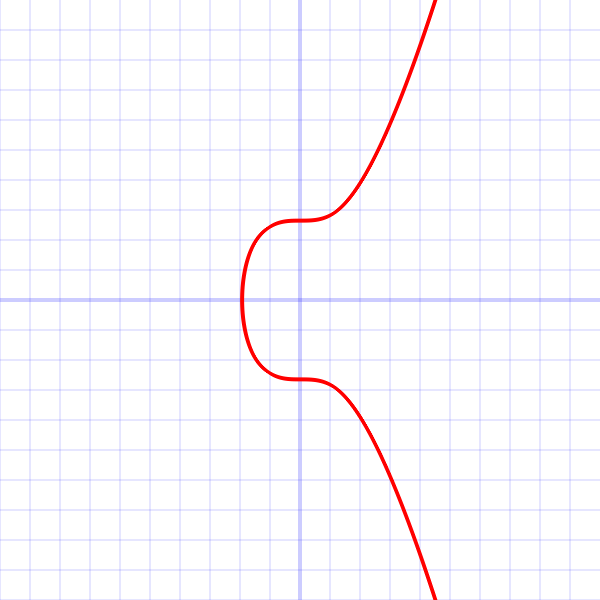
\includegraphics[width=0.35\textwidth]{images/Secp256k1.png}
    \caption{Gráfica de la curva \emph{secp256k1}}
    \label{im:secp256k1}
\end{figure}

Este algoritmo es el siguiente:

\begin{minipage}{0.9\textwidth}
    \begin{algorithm}[H] \label{alg:maptogroup}
        \caption{Nothing Up My Sleeve: MapToGroup}
        \KwIn{La cadena de entrada $m$ y el módulo primo de campo $p$.}
        \KwOut{Un punto de curva elíptica si tiene éxito o algún error.}
        $i = 0$ \\
        \While{$i < 256$}{
            $x = \operatorname{Hash}(m || i)$ \\
            $rhs = x^{3} + 7 (\operatorname{mod} \text{ p})$ \\
            \If{$rhs$ es un cuadrado $(mod$ $p)$}{
                $y = \sqrt{rhs}$ $(\operatorname{mod} p)$ \\
                \If{$(x, y)$ no es el punto en el infinito}{
                    \Return{$(x, y)$}
                }
            }
            $i = i+1$
        }
        \Return{``No se puede asignar al grupo''}
    \end{algorithm}
\end{minipage}

\begin{minipage}{0.9\textwidth}
    \begin{algorithm}[H] \label{alg:computegenerators}
        \caption{Computa Generadores: ComputeGenerators}
        \KwIn{La curva elíptica pública generadora $g \in \mathbb{G}$ y un entero $n$.}
        \KwOut{El conjunto de generadores $(g, h, \mathbf{g}, \mathbf{h})$}
        Computa $h = \operatorname{MapToGroup}($'algún string público', $p)$. \\
        $i = 0$ \\
        \While{$i < n$}{
            $c \in_{R} \mathbb{Z}_{p}$ \\
            $d \in_{R} \mathbb{Z}_{p}$ \\
            $\mathbf{g}[i] = c.G$ \\
            $\mathbf{h}[i] = d.G$ \\
            $i = i + 1$
        }
        \Return{$(g, h, \mathbf{g}, \mathbf{h})$}
    \end{algorithm}
\end{minipage}

Con esto, la configuración queda de la siguiente forma:

\begin{minipage}{0.9\textwidth}
    \begin{algorithm}[H]
        \caption{$\operatorname{Setup_{IP}}$}
        \KwIn{El conjunto de generadores $(g, h, \mathbf{g}, \mathbf{h})$.}
        \KwOut{$\operatorname{params_{IP}}$}
        $u = \operatorname{MapToGroup}($'algún string público', $p)$. \\
        \Return{$\operatorname{params_{IP}} = (g, h, \mathbf{g}, \mathbf{h}, u)$}
    \end{algorithm}
\end{minipage}

\begin{minipage}{0.9\textwidth}
    \begin{algorithm}[H]
        \caption{$\operatorname{Setup_{RP}}$}
        \KwIn{La curva elíptica pública generadora $g \in \mathbb{G}$ y un entero $n$.}
        \KwOut{$\operatorname{params_{RP}}$}
        \uIf{$b$ no es una potencia de $2$}{
            \Return{``$b$ tiene que ser una potencia de $2$''}
        }\Else{
            $n = \log_{2}(b)$ \\
            $(g, h, \mathbf{g}, \mathbf{h}) = \operatorname{ComputeGenerators}(g, n)$ \\
            $\operatorname{params_{IP}} = \operatorname{SetUp_{IP}}(g, h, \mathbf{g}, \mathbf{h})$ \\
            $\operatorname{params_{RP}} = \operatorname{(params_{IP}, n)}$ \\
            \Return{$\operatorname{params_{RP}}$}
        }
    \end{algorithm}
\end{minipage}

\subsubsection{Argumento del producto interno}

En esta sección presentamos el bloque de construcción principal de Bulletproofs, que es el argumento del producto interno. En resumen, utilizando este protocolo ZKP, el probador convence a un verificador de que conoce vectores cuyo producto interno es igual a un valor público determinado. Primero describimos el procedimiento de inicialización en el siguiente algoritmo:

\begin{minipage}{0.9\textwidth}
    \begin{algorithm}[H]
        \caption{Compromiso de vectores: $\operatorname{Commit_{IP}}$}
        \KwIn{$(\operatorname{params_{IP}}, \mathbf{a}, \mathbf{b})$}
        \KwOut{El compromiso $P$.}
        $P = g^{a}h^{b} \in \mathbb{G}$ \\
        \Return{$P$}
    \end{algorithm}
\end{minipage}

\begin{minipage}{0.9\textwidth}
    \begin{algorithm}[H]
        \caption{Prueba de Producto Interno: $\operatorname{Prove_{IP}}$}
        \KwIn{$(\operatorname{params_{IP}}, \operatorname{commit_{IP}}, c, \mathbf{a}, \mathbf{b})$}
        \KwOut{$\operatorname{proof_{IP}}$}
        $x = \operatorname{Hash}(\mathbf{b}, \mathbf{h}, P, c) \in \mathbb{Z}^{*}_{p}$ \\
        $P' = u^{x.c}P$ \\
        Asignar arrays $l, r \in \mathbb{G}^{n}$ \\
        $\operatorname{ComputeProof}(\mathbf{g}, \mathbf{h}, P', u^{x}, \mathbf{a}, \mathbf{b}, \mathbf{l}, \mathbf{r})$ \\
        $\operatorname{proof_{IP}} = (\mathbf{g}, \mathbf{h}, P', u^{x}, \mathbf{a}, \mathbf{b}, \mathbf{l}, \mathbf{r})$ \\
        \Return{$\operatorname{proof_{IP}}$}
    \end{algorithm}
\end{minipage}

Luego presentamos el protocolo principal, dado por el siguiente algoritmo:

\begin{minipage}{0.9\textwidth}
    \begin{algorithm}[H]
        \caption{Prueba de Producto Interno: $\operatorname{ComputeProof}$}
        \KwIn{$(\mathbf{g}, \mathbf{h}, P, u, a, b, \mathbf{l}, \mathbf{r})$}
        \KwOut{$(\mathbf{g}, \mathbf{h}, P, u, a, b, \mathbf{l}, \mathbf{r})$}
        $x = \operatorname{Hash}(\mathbf{g}, \mathbf{h}, P, c) \in \mathbb{Z}^{*}_{p}$ \\
        $P' = u^{x.c}P$ \\
        \uIf{$n == 1$}{
            \Return{$(\mathbf{g}, \mathbf{h}, P, u, a, b, \mathbf{l}, \mathbf{r})$}
        }\Else{
            $n' = \frac{n}{2}$ \\
            $C_{L} = <\mathbf{a}_{[:n']}, \mathbf{b}_{[n':]}> \in \mathbb{Z}_{p}$ \\
            $C_{R} = <\mathbf{a}_{[n':]}, \mathbf{b}_{[:n']}> \in \mathbb{Z}_{p}$ \\
            $L = \mathbf{g}_{[n':]}^{\mathbf{a}_{[:n']}} \mathbf{h}_{[:n']}^{\mathbf{b}{[n':]}}u^{c_{L}} \in \mathbb{G}$ \\
            $R = \mathbf{g}_{[:n']}^{\mathbf{a}_{[n':]}} \mathbf{h}_{[n':]}^{\mathbf{b}{[:n']}}u^{c_{R}} \in \mathbb{G}$ \\
            Añadir $L, R$ a $\mathbf{l}, \mathbf{r}$ respectivamente. \\
            $x = \operatorname{Hash}(L, R)$ \\
            $\mathbf{g}' = \mathbf{g}_{[:n']}^{x^{-1}} \mathbf{g}_{[n':]}^{x} \in \mathbb{G}^{n'}$ \\
            $\mathbf{h}' = \mathbf{g}_{[:n']}^{x} \mathbf{g}_{[n':]}^{x^{-1}} \in \mathbb{G}^{n'}$ \\
            $P' = L^{x^{2}}PR^{x^{-2}} \in \mathbb{G}$ \\
            $\mathbf{a}' = \mathbf{a}_{[:n']}x + \mathbf{a}_{[n':]}x^{-1} \in \mathbb{Z}_{p}^{n'}$ \\
            $\mathbf{b}' = \mathbf{b}_{[:n']}x^{-1} + \mathbf{b}_{[n':]}x \in \mathbb{Z}_{p}^{n'}$ \\
            Ejecutar recursivamente $\operatorname{ComputeProof}$ en $(\mathbf{g}', \mathbf{h}', P', u, \mathbf{a}', \mathbf{b}', \mathbf{l}, \mathbf{r})$
        }
    \end{algorithm}
\end{minipage}

\begin{minipage}{0.9\textwidth}
    \begin{algorithm}[H]
        \caption{Prueba de Producto Interno: $\operatorname{Verify_{IP}}$}
        \KwIn{$\operatorname{params_{IP}}, \operatorname{commit_{IP}}, \operatorname{proof_{IP}}$}
        \KwOut{True o False}
        $i = 0$ \\
        \While{$i < \log(n)$}{
            $n' = \frac{n}{2}$ \\
            $x = \operatorname{Hash}(\mathbf{l}[i], \mathbf{r}[i])$ \\
            $\mathbf{g}' = \mathbf{g}_{[:n']}^{x^{-1}} \mathbf{g}_{[n':]}^{x} \in \mathbb{G}^{n'}$ \\
            $\mathbf{h}' = \mathbf{g}_{[:n']}^{x} \mathbf{g}_{[n':]}^{x^{-1}} \in \mathbb{G}^{n'}$ \\
            $P' = L^{x^{2}}PR^{x^{-2}} \in \mathbb{G}$ \\
            $i = i+1$
        }
        El verificador calcula $c = a.b$ y acepta si $P = g^{a}h^{b}u^{c}$
    \end{algorithm}
\end{minipage}

El hecho de que Bulletproofs permita reducir a la mitad el tamaño del problema en cada nivel de recursión en el algoritmo $\operatorname{ComputeProof}$ significa que es posible obtener un tamaño de prueba logarítmico.

\subsubsection{Argumento de prueba de rango}

Dado un valor secreto $v$, si queremos probar que pertenece al intervalo $[0, 2^{n})$, tenemos que hacer lo siguiente:

\begin{itemize}
    \item Probar que $\mathbf{a}_{L} \in {0, 1}^{n}$ es la descomposición en bits de $v$. En otras palabras, tenemos que probar que:
    $$<\mathbf{a}_{L}, \mathbf{2}^{n}> = v$$

    \item Definir $\mathbf{a}_{R}$ como el complemento por componentes de $\mathbf{a}_{L}$, lo que significa que, por cada $i \in [0, n]$, si el $i$-ésimo bit de $\mathbf{a}_{L}$ es 0, entonces el $i$-ésimo bit de $\mathbf{a}_{R}$ es 1; y si el $i$-ésimo bit de $\mathbf{a}_{L}$ es 1, entonces el $i$-ésimo bit de $\mathbf{a}_{R}$ es 0.

    Equivalentemente, esta condición se puede expresar como:
    $$\mathbf{a}_{L} \circ \mathbf{a}_{R} = \mathbf{0}^{n}$$
    $$\mathbf{a}_{R} = \mathbf{a}_{L} - 1^{n} (\operatorname{mod} 2)$$

    Para probar que $\mathbf{a}_{L}$ y $\mathbf{a}_{R}$ satisfacen ambas relaciones podemos seleccionar de forma aleatoria un elemento $y \in \mathbb{Z}_{p}$ y computar:
    $$<\mathbf{a}_{L}, \mathbf{a}_{R} \circ \mathbf{y}^{n}> = 0$$
    $$<\mathbf{a}_{L} - \mathbf{1}^{n} - \mathbf{a}_{R}, \mathbf{y}^{n}> = 0$$

    Estas dos ecuaciones pueden ser combinadas en un único producto interno seleccionando un elemento aleatorio $z \in \mathbb{Z}_{p}$, y computando:
    $$<\mathbf{a}_{L} - z.\mathbf{1}^{n}, \mathbf{y}^{n} \circ (\mathbf{a}_{R} + z.\mathbf{1}^{n}) + z^{2}.\mathbf{2}^{n}> = z^{2}v + \delta(y, z)$$
    donde $\delta(y, z) = (z - z^{2})<\mathbf{1}^{n}, \mathbf{y}^{n}> - z^{3}<\mathbf{1}^{n}, \mathbf{2}^{n}> \in \mathbb{Z}_{p}$.
\end{itemize}

Si el probador pudiése enviar los vectores en la ecuación anterior, entonces el verificador será capaz de comprobar el producto interno él mismo. Sin embargo, este vector revela informacion sobre $\mathbf{a}_{L}$, por lo tanto revelando bits del valor secreto $v$. Para solucionar este problema, el proveder aleatoriamente elige vecores $\mathbf{s}_{L}$ y $\mathbf{s}_{R}$ para esconder $\mathbf{a}_{L}$ y $\mathbf{a}_{R}$ respectivamente. Considerando los siguientes polinimios:
$$l[X] = \mathbf{a}_{L} - z.1^{n} + s_{L}.X \in \mathbb{Z}_{p'}^{n}$$
$$r[X] = \mathbf{y^{n}} \circ (\mathbf{a}_{R} + z.1^{n} + \mathbf{s}_{R}.X) + z^{2}2^{n} \in \mathbf{Z}_{p'}^{n}$$
$$t[X] = <l[X], r[X]> = t_{0} + t_{1}.X + t_{2}.X^{2}$$
donde el producto interno anterior es computado como:
$$<\mathbf{l}(X), \mathbf{r}(X)> = \sum_{i=0}^{d} \sum_{j=0}^{i} <\mathbf{l}_{i}, \mathbf{r}_{j}>X^{i+j} \in \mathbb{Z}_{p}[X]$$

Tenga en cuenta que los términos constantes de $l[X]$ y $r[X]$ corresponden a los vectores en la ecuación previa:
$$<\mathbf{a}_{L} - z.\mathbf{1}^{n}, \mathbf{y}^{n} \circ (\mathbf{a}_{R} + z.\mathbf{1}^{n}) + z^{2}.\mathbf{2}^{n}> = z^{2}v + \delta(y, z)$$
Por lo tanto, si el probador publica $l[X]$ y $r[X]$ para un $x \in \mathbb{Z}_{p}$ específico, entonces tenemos que los términos $\mathbf{s}_{L}$ y $\mathbf{s}_{R}$ aseguran que no se revele información sobre $\mathbf{a}_{L}$ y $\mathbf{a}_{R}$.
Explicitamente tenemos que:
$$t_{1} = <\mathbf{a}_{L} - z.\mathbf{1}^{n}, \mathbf{y}^{n}.\mathbf{s}_{R})> + <\mathbf{s}_{L}, \mathbf{y}^{n}.(\mathbf{a}_{R} + z.\mathbf{1}^{n}>$$
$$t_{2} = <\mathbf{s}_{L}, \mathbf{y}^{n}.\mathbf{s}_{R}>$$

Finalmente, tenemos que el algoritmo es el siguiente:

\begin{minipage}{0.9\textwidth}
    \begin{algorithm}[H]
        \caption{Bulletproofs: $\operatorname{Prove_{RP}}$}
        \KwIn{$\operatorname{params_{RP}}, v$}
        \KwOut{$\operatorname{proof_{RP}}$}
        $\gamma \in_{R} \mathbb{Z}_{p}$ \\
        $V = g^{v}h^{\gamma} \in \mathbb{G}$ \\
        $\mathbf{a}_{L}\in \{0, 1\}^{n}$ tal que $<\mathbf{a}_{L}, \mathbf{2}^{n}> = v$ \\
        $\mathbf{a}_{R} = \mathbf{a}_{L} - \mathbf{1}^{n} \in \mathbb{z}_{p}^{n}$ \\
        $\alpha \in_{R} \mathbb{Z}_{p}$ \\
        $A = h^{\alpha}\mathbf{g}^{\mathbf{a}_{L}}\mathbf{h}^{\mathbf{a}_{R}} \in \mathbb{G}$ \\
        $s_{L}, s_{R} \in_{R} \mathbb{Z}_{p}^{n}$ \\
        $\rho \in_{R} \mathbb{Z}_{p}$ \\
        $S = h^{\rho}\mathbf{g}^{s_{L}}\mathbf{h}^{s_{R}} \in \mathbb{G}$ \\
        $y = \operatorname{Hash}(A, S) \in \mathbb{Z}_{p}^{*}$ \\
        $z = \operatorname{Hash}(A, S, y) \in \mathbb{Z}_{p}^{*}$ \\
        $\tau_{1}, \tau_{2} \in_{R} \mathbb{Z}_{p}$ \\
        $T_{1} = g^{t_{1}}h^{\tau_{1}} \in \mathbb{G}$ \\
        $T_{2} = g^{t_{2}}h^{\tau_{2}} \in \mathbb{G}$ \\
        $x = \operatorname{Hash}(T_{1}, T_{2}) \in \mathbb{Z}_{p}^{*}$ \\
        $\mathbf{l} = l(X) = \mathbf{a}_{L} - z1^{n} + s_{L}X \in \mathbb{Z}_{p}^{n}$ \\
        $\mathbf{r} = r(X) = \mathbf{y}^{n} \circ (\mathbf{a}_{R} + z1^{n}+s_{R}X) + z^{2}2^{n} \in \mathbb{Z}_{p}^{n}$ \\
        $\hat{t} = <\mathbf{l}, \mathbf{r}> \in \mathbb{Z}_{p}$ \\
        $\tau_{x} = \tau_{2}x^{2} + \tau_{1}x + z^{2}\gamma \in \mathbb{Z}_{p}$ \\
        $\mu = \alpha + \rho x \in \mathbb{Z}_{p}$ \\
        $\operatorname{commit_{IP}} = \operatorname{Commit_{IP}}(\operatorname{params_{IP}}, \mathbf{l}, \mathbf{r})$ \\
        $\operatorname{proof_{IP}} = \operatorname{Prove_{IP}}(\operatorname{params_{IP}}, \operatorname{commit_{IP}}, \hat{t}, \mathbf{l}, \mathbf{r})$ \\
        $\operatorname{proof_{RP}} = (\tau_{x}, \mu, \hat{t}, V, A, S, T_{1}, T_{2}, \operatorname{commit_{IP}}, \operatorname{proof_{IP}})$ \\
        \Return{$\operatorname{proof_{RP}}$}
    \end{algorithm}
\end{minipage}

\begin{minipage}{0.9\textwidth}
    \begin{algorithm}[H]
        \caption{Bulletproofs: $\operatorname{Verify_{RP}}$}
        \KwIn{$\operatorname{params_{RP}}, \operatorname{proof_{RP}}$}
        \KwOut{True o False.}
        $y = \operatorname{Hash}(A, S) \in \mathbb{Z}_{p}^{*}$ \\
        $z = \operatorname{Hash}(A, S, y) \in \mathbb{Z}_{p}^{*}$ \\
        $x = \operatorname{Hash}(T_{1}, T_{2}) \in \mathbb{Z}_{p}^{*}$ \\
        $h_{i} = h_{i}^{y^{-i+1}} \in \mathbb{G}, \forall i \in [1, n]$ \\
        $P_{l} = P.h^{\mu}$ \\
        $P_{r} = A.S^{x}.\mathbf{g}^{z}.(\mathbf{h}')^{z.\mathbf{y}^{n}+z^{2}.\mathbf{2}^{n}} \in \mathbb{G}$ \\
        $\operatorname{output_{1}} = (P_{l} == P_{r})$ \\
        $\operatorname{output_{2}} = (g^{\hat{t}h^{\tau_{x}}} == V^{z^{2}}.g^{\delta(y, z)}.T_{1}^{x}.T_{2}^{x^{2}})$ \\
        $\operatorname{output_{3}} = \operatorname{Verify_{IP}}(\operatorname{proof_{IP}}$ \\
        \Return{$\operatorname{output_{1}} \wedge \operatorname{output_{2}} \wedge \operatorname{output_{3}}$}
    \end{algorithm}
\end{minipage}

\section{Selección de algoritmo} \label{sec:seleccion}

Para elegir el algoritmo en el que centraremos el estudio, comparemos los algoritmos \emph{Multi-base}, \emph{Descomposición Cuadrada} (\emph{Square Decomposition}), \emph{Basado en firma} (\emph{Signature-based}) y \emph{Bulletproofs} desarrollados previamente.

Lo primero que se considera a la hora de elegir el algoritmo que vamos a desarrollar es ver cuál de ellos es más eficiente. Para ello, se estudia cómo afecta el tamaño de las pruebas a la complejidad en bits, y cómo afecta el tamaño de las pruebas a la complejidad en tiempo para el probador y el verificador.

\begin{figure}[H]
    \centering
    \begin{subfigure}[c]{0.45\textwidth}
        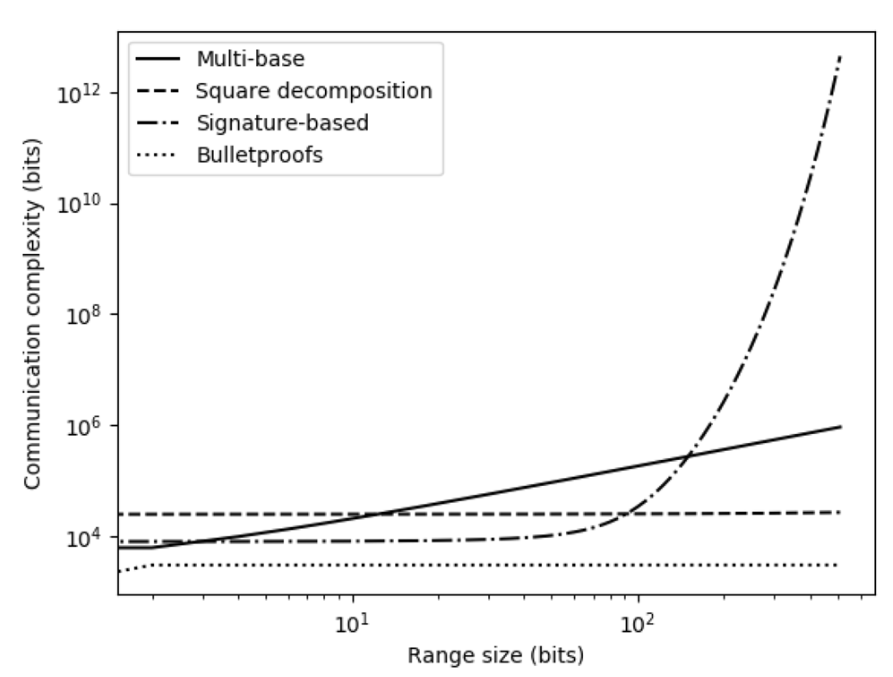
\includegraphics[width=\textwidth]{images/proofsSize.png}
        \caption{Tamaño de las pruebas}
    \end{subfigure}
    
    \begin{subfigure}[c]{0.45\textwidth}
        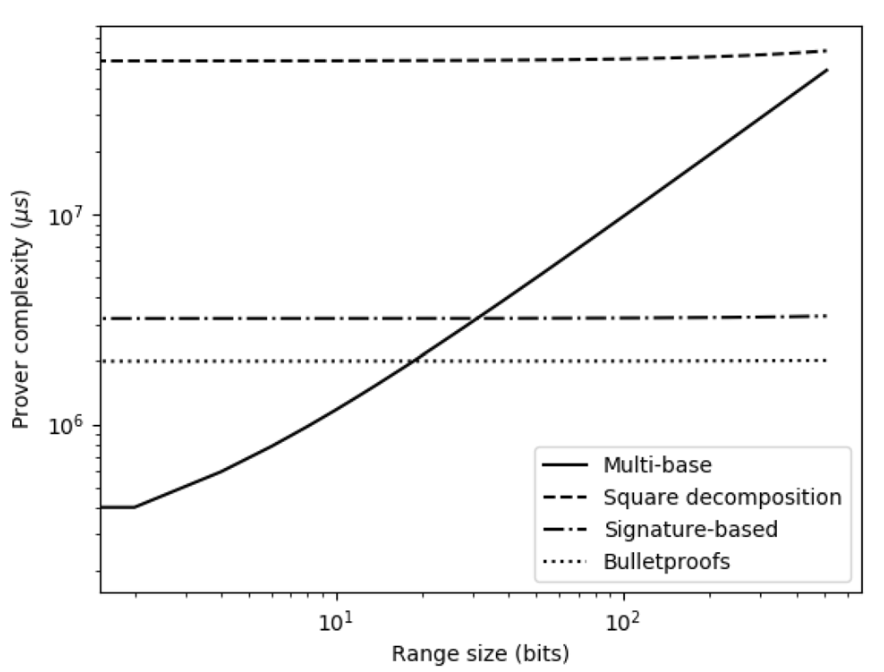
\includegraphics[width=\textwidth]{images/proverComplexity.png}
        \caption{Complejidad del probador}
    \end{subfigure}
    \begin{subfigure}[c]{0.45\textwidth}
        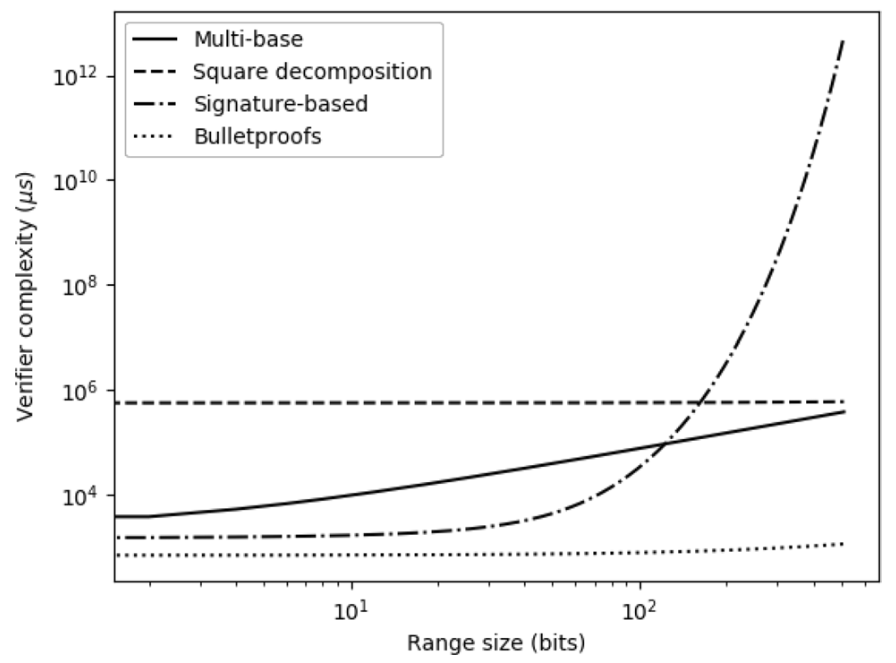
\includegraphics[width=\textwidth]{images/verifierComplexity.png}
        \caption{Complejidad del verificador}
    \end{subfigure}
    \caption{Comparación entre los distintos algoritmos \cite{Survey}}
    \label{im:comparacion}
\end{figure}

Se puede ver que los dos algoritmos más interesantes son \emph{Bulletproofs} y \emph{Descomposición Cuadrada}, ya que al aumentar el tamaño de la prueba la complejidad en bits y la complejidad en tiempo del probador y el verificador se mantienen casi constante. Esto permite descartar los algoritmos \emph{Signature-based} y \emph{Multi-base}.

También es interesante comparar ahora \emph{Bulletproofs} con los algoritmos \emph{ZK-STARKS} y \emph{ZK-SNARKS} estudiados brevemente en \nameref{sec:clases}, donde tenemos:
\begin{figure}[H]
    \centering
    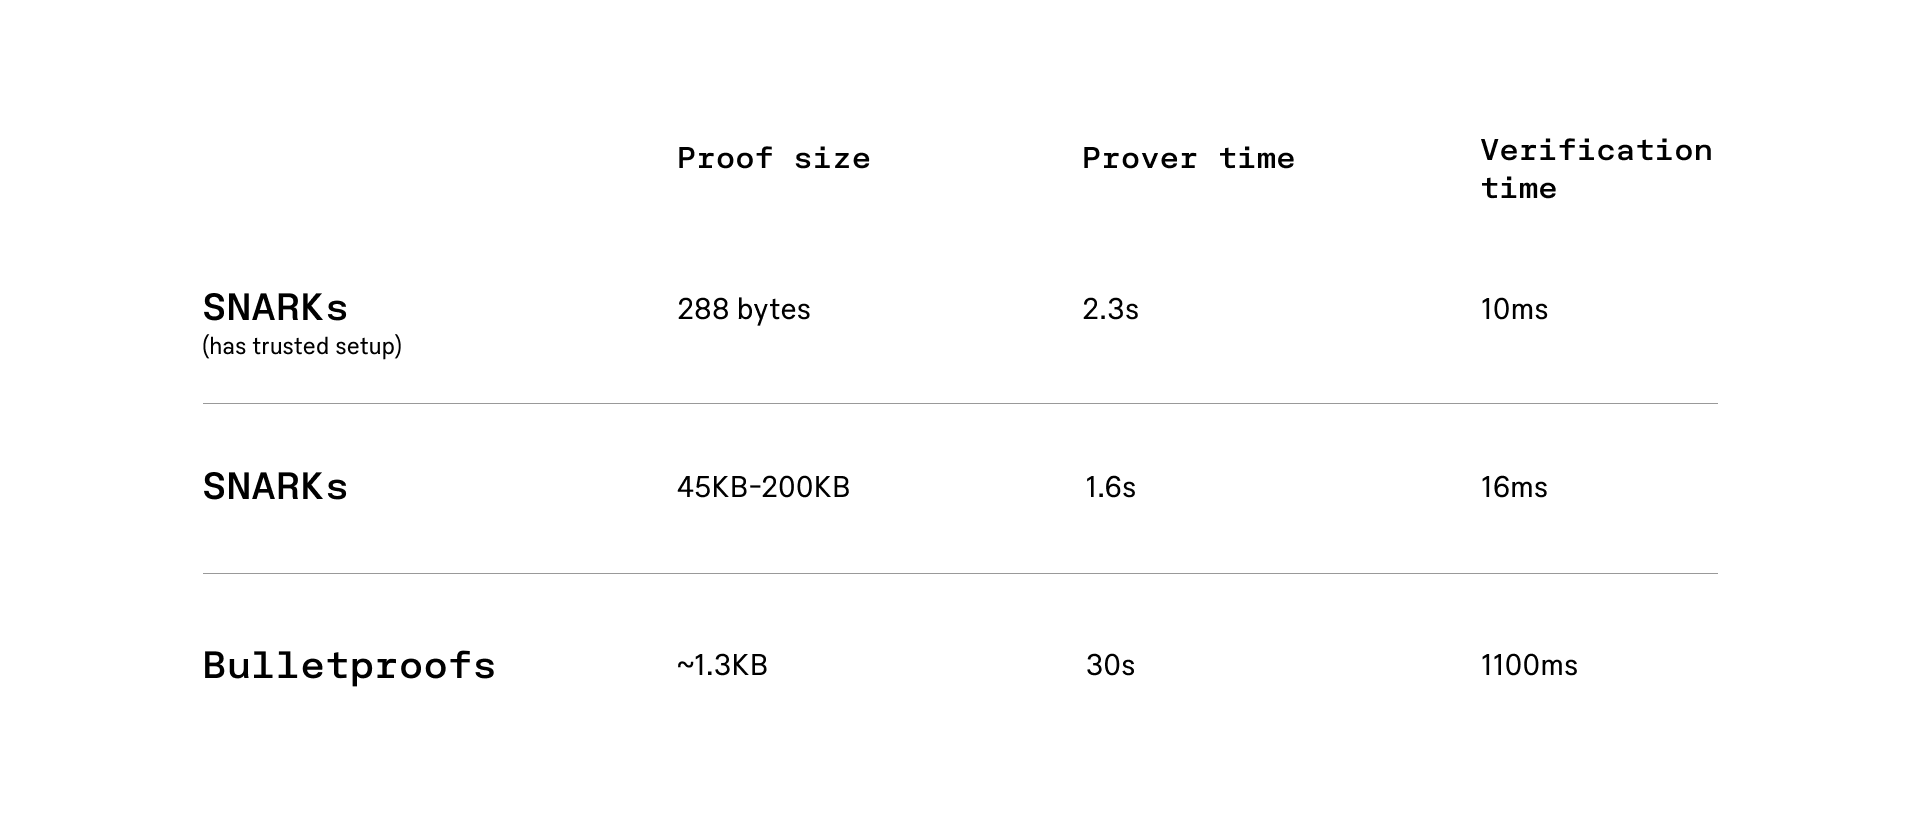
\includegraphics[width=\textwidth]{images/comparison2.png}
    \caption{Comparación entre Bulletproofs, ZK-STARKS y ZK-SNARKS \cite{Comparacion}}
\end{figure}

Es decir, tenemos el siguiente esquema:
\begin{figure}[H]
    \centering
    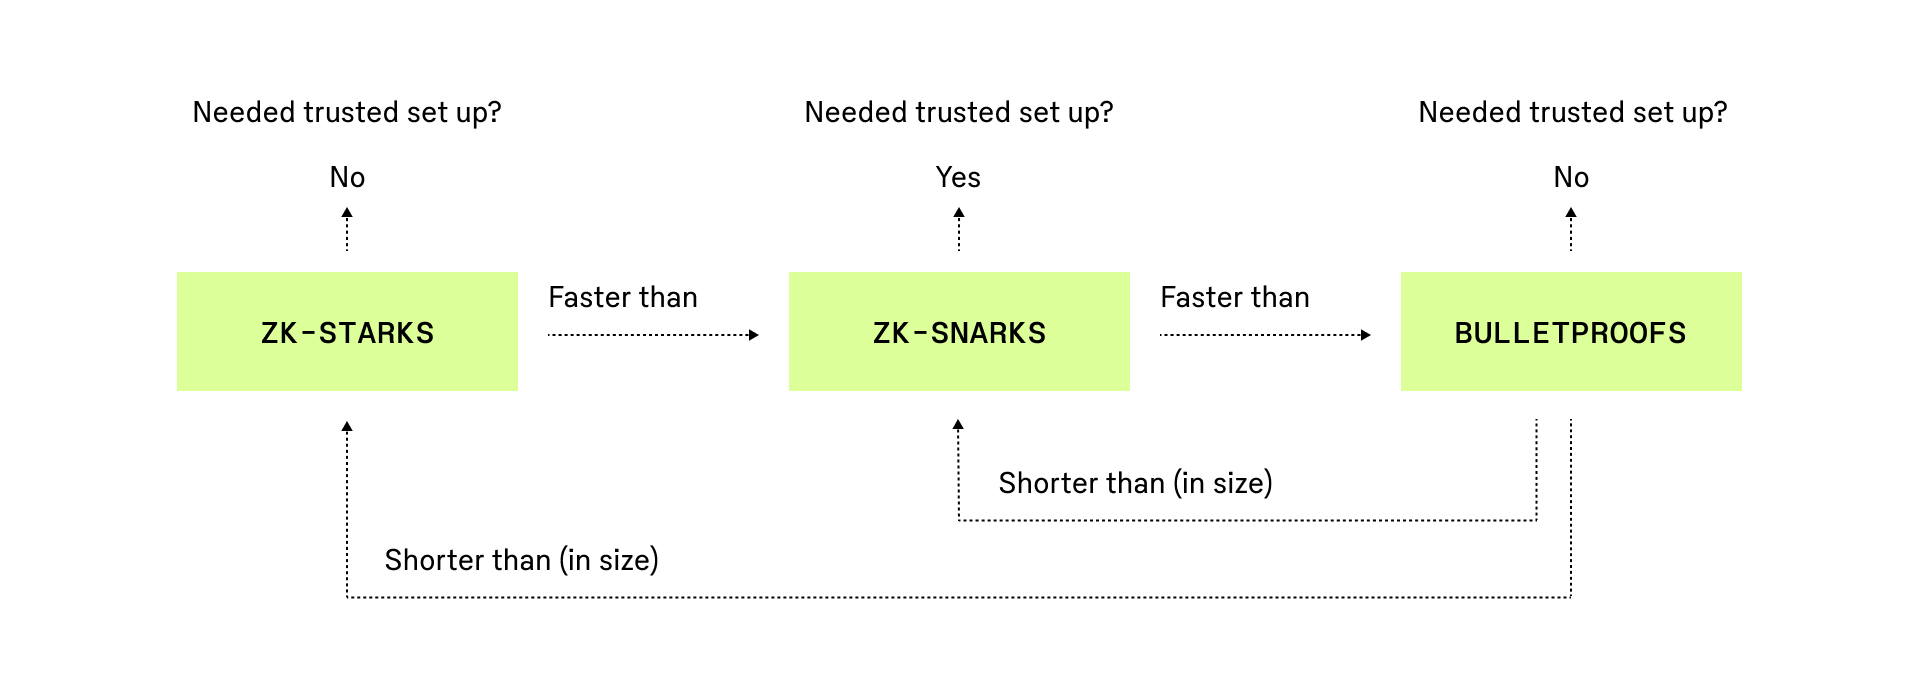
\includegraphics[width=\textwidth]{images/comparison.png}
    \caption{Comparación entre Bulletproofs, ZK-STARKS y ZK-SNARKS \cite{Comparacion}}
\end{figure}

Y como se vio en la \autoref{im:comparacion}, el algoritmo \emph{Descomposición Cuadrada} funciona similar a las \emph{Bulletproofs}, pero más lento y con una complejidad de mayor tamaño.

Como los \emph{Bulletproofs} no requieren establecimiento de confianza y son menores en tamaño, aunque sean algo más lentos, es uno de los algoritmos más interesantes hoy en día, y el principal que consideramos como objeto de este estudio. Sin embargo, debido a la complejidad de dicho algoritmo y que nuestro objetivo es facilitar la comprensión de los protocolos de conocimiento cero, decidimos centrarnos en uno más simple, la \emph{Descomposición Cuadrada}, ya que es más fácil comprender su funcionamiento utilizando la herramienta que desarrollaremos. Además, en septiembre del 2022 se publicó un artículo, \emph{Sharp: Short Relaxed Range Proofs} por Geoffroy Couteau, Dahmun Goudarzi, Michael Klooß y
Michael Reichle \cite{Sharp}, que presenta un nuevo algoritmo, Sharp, basado en la \emph{Descomposición cuadrada} y cuyas pruebas son casi un 50\% más cortas que las de \emph{Bulletproof}, lo cual nos da incluso más motivos para seleccionar este algoritmo.

\begin{figure}[H]
    \centering
    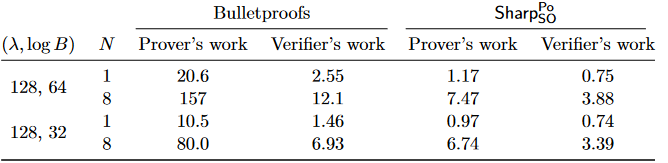
\includegraphics[width=\textwidth]{images/sharp vs bulletproof.png}
    \caption{Comparación en milisegundos entre SHARP y Bulletproofs \cite{Sharp}}
\end{figure}
